\chapter{Materiales y Métodos}
\label{chap:materiales_metodos}

\noindent Este capítulo detalla la metodología empleada en la investigación, incluyendo el diseño del estudio, la selección del dispositivo \textit{wearable}, el protocolo de reclutamiento de participantes, la extracción y preprocesamiento de datos biométricos, el desarrollo de variables derivadas mediante ingeniería de características, el establecimiento de la verdad operativa mediante \textit{clustering} no supervisado, el diseño del sistema de inferencia difusa tipo \textit{Mamdani}, y el protocolo de validación cruzada \textit{Leave-One-User-Out}. Describimos el procedimiento completo desde la aprobación ética inicial hasta la validación final del modelo, lo cual facilita la comprensión del proceso metodológico y garantiza la reproducibilidad de los hallazgos en estudios futuros. Cada sección se enlaza con la anterior mediante transiciones explícitas que guían al lector a través del flujo lógico de decisiones metodológicas implementadas.

% ═══════════════════════════════════════════════════════════════════════════
% BLOQUE 1: DISEÑO Y PLANIFICACIÓN
% ═══════════════════════════════════════════════════════════════════════════

% ============================================================================
\section{Diseño del Estudio y Aprobaciones Éticas}
\label{sec:diseno}
% ============================================================================

Empleamos un diseño cuantitativo con enfoque exploratorio-correlacional, de tipo longitudinal retrospectivo con seguimiento multianual (2021-2024) de una cohorte de 10 participantes adultos, de naturaleza observacional de un solo corte y sin grupo control. El componente exploratorio del estudio reside en el descubrimiento de patrones latentes de comportamiento sedentario mediante técnicas de \textit{clustering} no supervisado aplicadas a datos biométricos recolectados en condiciones de vida libre, mientras que el componente correlacional se manifiesta en la validación de la concordancia entre dos métodos independientes: la clasificación obtenida mediante agrupamiento \textit{K-Means} y la clasificación generada por el sistema de inferencia difusa \textit{Mamdani}. Este diseño se fundamenta en el paradigma \textit{Bring Your Own Device} (\textit{BYOD}), el cual minimiza el efecto Hawthorne al utilizar dispositivos que los participantes ya poseían y empleaban regularmente en su vida cotidiana, garantizando validez en condiciones naturales de actividad \cite{Doherty2021}.

El protocolo de investigación fue sometido a escrutinio y aprobación por parte del Comité de Investigación y el Comité de Ética en Investigación de la Facultad de Medicina y Ciencias Biomédicas de la Universidad Autónoma de Chihuahua. Obtuvimos el primer dictamen favorable del Comité de Investigación el 17 de febrero de 2025, documentado mediante el Oficio SIP/116/25 con asignación de registro interno de proyecto CI-088-24. Posteriormente, el Comité de Ética en Investigación aprobó el protocolo completo el 21 de agosto de 2025 bajo el mismo número de registro CI-088-24, lo cual nos permitió lanzar la convocatoria abierta para reclutamiento de participantes a partir de esa fecha. El estudio se estructuró en un seguimiento retrospectivo que abarcó datos biométricos recopilados de forma continua por los participantes durante sus actividades diarias habituales, con una mediana de seguimiento de 131 semanas por participante. La unidad de análisis correspondió a semanas completas de monitoreo, las cuales generamos mediante la agregación temporal de los 9,185 días válidos recopilados de forma continua por los dispositivos \textit{Apple Watch}, decisión metodológica que fundamentamos en la necesidad de reducir el ruido inherente a las mediciones diarias en condiciones de vida libre mediante estadísticos robustos, como desarrollaremos en la Sección~\ref{subsec:agregacion_semanal}.

% ============================================================================
\section{Selección del Dispositivo Wearable}
\label{sec:seleccion_dispositivo}
% ============================================================================

Para la selección del dispositivo de monitoreo, utilizamos una base de datos detallada que analiza 423 dispositivos de 133 marcas, divididos en 187 monitores de actividad física y 236 relojes inteligentes lanzados desde 2011 \cite{Henriksen2021ReplicationData}. Esta base nos permitió identificar las capacidades técnicas de cada dispositivo, como sensores incluidos y su utilidad en la medición de patrones de actividad física (AF) y comportamiento sedentario (CS). Del análisis de los 423 dispositivos, identificamos que todos cuentan con acelerómetro triaxial, esencial para medir la intensidad y frecuencia del movimiento. Sin embargo, solo el 38.3\% de los dispositivos (162 de 423) incluyen un sensor de fotopletismografía (PPG), crucial para medir frecuencia y variabilidad cardíaca, indicadores relevantes para evaluar esfuerzo físico y salud cardiovascular \cite{Pinto2023Physiology}.

El análisis de mercado identificó a Apple como el líder en la categoría de relojes inteligentes, con un 49\% de la cuota global, seguido por Samsung (15\%) y Garmin (11\%) \cite{Canalys2024Wearables}. Esta predominancia, combinada con reportes de disponibilidad en población urbana mexicana, motivó la inclusión de \textit{Apple Watch} como candidato prioritario en nuestra matriz de decisión. La \Cref{tab:wearables_comparison_extended} resume la matriz de decisión empleada para comparar los principales proveedores disponibles en México, incorporando criterios de penetración en el mercado nacional, validación científica de sensores, capacidad de exportación de datos históricos, consistencia entre versiones de hardware y software, y disponibilidad de \textit{SDK} (\textit{Software Development Kit}) o documentación técnica para desarrollo de herramientas de análisis personalizadas. La tabla nos ayuda a interpretar las características de cada proveedor por diferentes criterios, lo que permite identificar fortalezas y debilidades relativas y facilita elegir el dispositivo con mayor solidez técnica y disponibilidad para investigación en el contexto nacional.

\begin{table}[H]
    \centering
    \caption{Matriz de decisión extendida para selección de dispositivo wearable}
    \label{tab:wearables_comparison_extended}
    \begingroup
    \setlength{\tabcolsep}{4pt}
    \renewcommand{\arraystretch}{1.15}
    \fontsize{12}{14.4}\selectfont
    \begin{tabularx}{\textwidth}{@{}p{3.0cm}*{5}{>{\raggedright\arraybackslash}X}@{}}
        \toprule
        \textbf{Criterio} & \textbf{Apple Watch} & \textbf{Fitbit} & \textbf{Garmin} & \textbf{Polar} & \textbf{Huawei} \\
        \midrule
        Penetración en México & Alta & Media & Media-baja & Baja & Media \\
        Sensores validados & Sí (todos) & Sí (núcleo) & Sí (núcleo) & Sí (núcleo) & Parcial \\
        Exportación de datos & \textit{HealthKit} (\textit{XML}/\textit{API}) & Fitbit Web \textit{API} & Garmin Health \textit{API} & Polar AccessLink & Huawei Health \textit{API} (limitada) \\
        Consistencia HW/SW & Alta (ecosistema cerrado) & Media & Alta & Media & Baja (fragmentación) \\
        \textit{SDK} / Documentación & \textit{HealthKit} (extensa) & \textit{API} con foros activos & Documentación integral & Moderada (deportiva) & Limitada/básica \\
        \bottomrule
    \end{tabularx}
    \endgroup
\end{table}

\FloatBarrier

La comparación evidenció que \textit{Apple Watch} presenta ventajas decisivas en tres aspectos críticos para investigación científica: (1) ecosistema cerrado que garantiza alta consistencia entre versiones de hardware (Series 3 a 9) y actualizaciones de software, minimizando heterogeneidad instrumental; (2) función de exportación nativa mediante \textit{HealthKit} que proporciona el historial completo del usuario en formato XML estructurado, sin restricciones de antigüedad ni limitaciones de API; y (3) validación científica documentada en literatura que reporta concordancia superior al 90\% con estándares de referencia para frecuencia cardíaca y conteo de pasos \cite{Shcherbina2017}. Estas fortalezas técnicas, combinadas con la factibilidad de reclutamiento en la población objetivo mediante el paradigma BYOD (participantes que ya poseen el dispositivo), nos llevaron a seleccionar \textit{Apple Watch} como dispositivo estándar del estudio.

No obstante, reconocemos tres limitaciones inherentes a esta decisión que deben considerarse al interpretar los hallazgos: (1) sesgo de selección al excluir usuarios de plataformas Android u otros ecosistemas \textit{wearables}, lo cual limita la generalización poblacional; (2) barrera económica asociada al costo de los dispositivos Apple (USD \$300-800), que restringe la representatividad socioeconómica de la muestra al excluir participantes de estratos económicos sin acceso a esta tecnología; y (3) heterogeneidad entre versiones del \textit{Apple Watch} en métricas avanzadas, particularmente en análisis de sueño (Series 6+ vs Series 3-5), variabilidad cardíaca (Series 4+ con sensor óptico mejorado vs Series 3), electrocardiograma (disponible solo desde Series 4), y estimación de VO$_2$max (algoritmos refinados en versiones recientes), lo cual introduce variabilidad instrumental no controlada en estudios que incluyan dispositivos de múltiples generaciones. A pesar de estas limitaciones, el balance entre validez científica de los sensores, disponibilidad de datos históricos completos mediante función de exportación nativa, y factibilidad de reclutamiento bajo paradigma BYOD justifica la selección de \textit{Apple Watch} como dispositivo óptimo para los objetivos del presente estudio. Esta decisión metodológica determinó los procedimientos de extracción de datos que describimos en la siguiente sección.

% ============================================================================
\section{Protocolo de Convocatoria y Reclutamiento de Participantes}
\label{sec:convocatoria}
% ============================================================================

Tras obtener la aprobación del Comité de Ética en Investigación (registro CI-088-24, 21 de agosto de 2025), lanzamos una convocatoria abierta dirigida a estudiantes y personal de la Facultad de Medicina y Ciencias Biomédicas de la Universidad Autónoma de Chihuahua. Difundimos la invitación mediante dos canales complementarios: (1) publicaciones en redes sociales institucionales de la facultad, y (2) grupos de \textit{WhatsApp} de la facultad, canal ampliamente utilizado en la comunidad universitaria aunque no constituye un medio institucional formal. La convocatoria estuvo activa durante el período comprendido entre agosto y octubre de 2025, tiempo durante el cual recibimos manifestaciones de interés de 10 candidatos.

Establecimos criterios de inclusión específicos para garantizar la calidad y homogeneidad mínima de los datos: (1) propiedad y uso activo de un \textit{Apple Watch} Series 3 o superior, (2) uso continuo del dispositivo por un período mínimo de 6 meses previos a la fecha de reclutamiento para minimizar efectos de habituación y garantizar datos históricos suficientes, (3) edad entre 18 y 65 años, (4) capacidad ambulatoria sin limitaciones severas que impidieran actividad física cotidiana, y (5) disponibilidad y competencia técnica para exportar datos históricos completos del ecosistema \textit{HealthKit} mediante la función nativa de la aplicación \textit{Apple Health}. Los 10 candidatos que manifestaron interés cumplieron la totalidad de estos criterios de inclusión, obteniendo una tasa de elegibilidad del 100\%.

Diseñamos un proceso de reclutamiento y obtención de consentimiento informado completamente digital mediante una \textit{landing page} creada en \textit{Google Sites}. La \textit{landing page} contenía información detallada sobre los objetivos del estudio, los procedimientos de recolección de datos, los riesgos mínimos asociados (principalmente vinculados a la confidencialidad de información sensible de salud), las medidas de protección implementadas, y los derechos de los participantes incluyendo el retiro voluntario sin penalización en cualquier momento. Los participantes accedieron a esta plataforma digital donde: (1) revisaron la información completa del protocolo, (2) cargaron su archivo \path{export.zip} generado mediante la función de exportación nativa de \textit{Apple Health}, (3) completaron un formulario de \textit{Google Forms} con datos demográficos y antropométricos básicos, y (4) aceptaron los términos y condiciones del consentimiento informado de manera digital, cumpliendo con los lineamientos éticos establecidos en los Principios éticos para las investigaciones médicas en seres humanos de la Declaración de Helsinki, las Directrices para investigaciones relacionadas con la salud con seres humanos de las Pautas Éticas Internacionales del CIOMS, la normativa mexicana para investigaciones en salud del Reglamento de la Ley General de Salud en Materia de Investigación, y especialmente la legislación mexicana sobre protección de datos personales definida en la Ley General de Protección de Datos Personales en Posesión de Sujetos Obligados, esta última aplicable de forma nacional para la cesión de datos sensibles de salud.

Los 10 participantes que firmaron el consentimiento informado digital completaron exitosamente el protocolo de exportación de datos históricos. Dado que el estudio consistió en un análisis retrospectivo de datos históricos ya recolectados por los dispositivos durante el uso cotidiano de los participantes, no fue necesario que los usuarios permanecieran activos en monitoreo durante el período de investigación, sino únicamente que cumplieran el criterio de haber utilizado el \textit{Apple Watch} de forma continua durante al menos 6 meses previos, criterio que todos los participantes satisficieron. Esta cohorte final quedó conformada por 5 mujeres y 5 hombres (distribución balanceada por sexo), estableciendo las características demográficas que describimos en la siguiente sección.

% ============================================================================
\section{Características Demográficas de la Cohorte}
\label{sec:caracteristicas_cohorte}
% ============================================================================

La distribución balanceada por sexo (50\%/50\%) y el amplio rango de seguimiento en días de monitoreo continuo permiten capturar heterogeneidad inter-sujeto e intra-sujeto, características esenciales para evaluar la robustez del sistema de inferencia difusa en condiciones de vida libre. Presentamos las características detalladas en la \Cref{tab:cohorte_caracteristicas}.

\begin{table}[H]
\centering
\caption{Características demográficas y antropométricas de la cohorte (N=10)}
\label{tab:cohorte_caracteristicas}
\begingroup
\setlength{\tabcolsep}{5pt}
\renewcommand{\arraystretch}{1.1}
\small
\begin{tabular}{@{}lccccc@{}}
\toprule
\textbf{Usuario} & \textbf{Sexo} & \textbf{Edad (años)} & \textbf{IMC (kg/m²)} & \textbf{Días válidos} & \textbf{Completitud (\%)} \\
\midrule
u1 & F & 34 & 23.5 & 1,048 & 100 \\
u2 & F & 37 & 26.6 & 50    & 100 \\
u3 & F & 39 & 28.7 & 980   & 100 \\
u4 & M & 25 & 30.9 & 96    & 100 \\
u5 & F & 28 & 25.0 & 96    & 100 \\
u6 & M & 34 & 30.9 & 1,861 & 100 \\
u7 & M & 32 & 37.8 & 799   & 100 \\
u8 & M & 29 & 28.1 & 1,332 & 100 \\
u9 & M & 32 & 36.2 & 2,070 & 100 \\
u10 & F & 28 & 21.6 & 853   & 100 \\
\midrule
\textbf{Media$\pm$DE} & 5M/5F & 31.8$\pm$4.5 & 28.9$\pm$5.1 & 918.5$\pm$626.1 & 100 \\
\bottomrule
\end{tabular}
\endgroup
\end{table}

\FloatBarrier

La distribución etaria de la cohorte (rango 25-39 años, media 31.8$\pm$4.5 años) corresponde a adultos jóvenes en edad productiva, grupo demográfico de particular interés epidemiológico debido a que constituye la población económicamente activa susceptible a comportamiento sedentario ocupacional prolongado. El rango de índice de masa corporal observado (21.6-37.8 kg/m², media 28.9$\pm$5.1 kg/m²) abarca desde normopeso (IMC 18.5-24.9) hasta obesidad grado II (IMC 35.0-39.9) según la clasificación de la Organización Mundial de la Salud, proporcionando variabilidad antropométrica suficiente para evaluar si el sistema de clasificación de sedentarismo es robusto ante diferencias en composición corporal. El seguimiento temporal evidenció marcada heterogeneidad entre participantes en términos de días de monitoreo continuo: los 10 participantes generaron un total de 9,185 días válidos post-limpieza (media 918.5$\pm$626.1 días por participante), con rango desde 50 días (participante u2, seguimiento mínimo de aproximadamente 7 semanas) hasta 2,070 días (participante u9, seguimiento máximo de aproximadamente 298 semanas equivalentes a 5.7 años de monitoreo continuo).

Esta dispersión refleja diferencias en la antigüedad de adopción del \textit{Apple Watch} por cada usuario: participantes u6 y u9 contaban con datos históricos superiores a 5 años (1,861 y 2,070 días respectivamente), mientras que participantes u2, u4 y u5 habían incorporado el dispositivo a su uso cotidiano entre 3 y 4 meses antes del reclutamiento (50, 96 y 96 días válidos respectivamente). A pesar de esta disparidad, todos los participantes cumplieron el criterio mínimo de 6 meses de uso continuo (equivalente a aproximadamente 180 días), garantizando un período de habituación suficiente para que el dispositivo capturara patrones de comportamiento representativos del estilo de vida habitual, no de una fase de adaptación o novedad tecnológica. La completitud del 100\% (última columna de la \Cref{tab:cohorte_caracteristicas}) refleja que todos los días incluidos en el análisis cumplieron los criterios de calidad de datos establecidos en la Sección~\ref{sec:calidad_datos}. Estas características demográficas y antropométricas de la cohorte configuran el contexto dentro del cual justificamos el tamaño muestral empleado.

% ============================================================================
\section{Justificación del Tamaño Muestral}
\label{sec:justificacion_n}
% ============================================================================

Justificamos el tamaño final de N=10 participantes por el carácter longitudinal del diseño y la densidad de observaciones temporales generadas por cada participante. En diseños longitudinales densos, el poder estadístico no proviene exclusivamente del número de sujetos, sino del número total de observaciones temporales válidas disponibles para el modelado. Este enfoque se alinea con el paradigma de muestras densamente monitoreadas (\textit{intensive longitudinal designs}; \cite{Bolger2013}), donde el poder estadístico deriva del producto entre el número de participantes y las observaciones temporales promedio por sujeto:

\begin{equation}
\text{Poder} \propto N \times \bar{n}_{\text{obs/sujeto}}
\label{eq:poder_longitudinal}
\end{equation}

En nuestro estudio, cada participante generó datos diarios de forma continua mediante su \textit{Apple Watch}, los cuales consolidamos en un total de 9,185 días válidos post-limpieza. Estos días se agregaron temporalmente en semanas completas (ventana de 7 días consecutivos), aplicando el criterio de validez de ≥5 días con datos completos por semana. Este proceso generó 1,385 semanas candidatas, de las cuales 1,337 cumplieron el criterio de validez, resultando en un promedio de 133.7 semanas válidas por participante (mediana: 131 semanas; rango: 7-298 semanas). Con N=10 participantes y $\bar{n}_{\text{obs}}$=133.7 semanas, el cálculo de poder según la Ecuación~\ref{eq:poder_longitudinal} arroja $n_{\text{total}}=1{,}337$ observaciones semanales, valor que supera ampliamente el mínimo recomendado de $n_{\text{total}} \geq 500$ para algoritmos de agrupamiento estable y validación cruzada robusta \cite{Alinia2020}.

Este total de 1,337 observaciones semanales independientes proporciona suficiente poder para la validación cruzada mediante la estrategia \textit{Leave-One-User-Out}, donde cada participante sirve como conjunto de prueba una vez mientras los 9 restantes conforman el conjunto de entrenamiento. La riqueza informativa de este diseño longitudinal denso supera considerablemente la que se obtendría en un estudio transversal con 1,337 participantes individuales medidos una sola vez, ya que las mediciones repetidas dentro de cada sujeto permiten capturar tanto variabilidad inter-sujeto (entre participantes) como variabilidad intra-sujeto (fluctuaciones temporales dentro del mismo individuo), ambas esenciales para evaluar la robustez del sistema de clasificación en condiciones reales de vida libre donde el comportamiento sedentario no es estable día a día. La distribución del seguimiento entre participantes mostró alta variabilidad (CV=68\%), con usuarios monitoreados desde 50 días (seguimiento mínimo, participante u2) hasta 2,070 días (seguimiento máximo, participante u9), heterogeneidad temporal que constituye una fortaleza metodológica al permitir evaluar la robustez del sistema de inferencia difusa en condiciones diversas de duración de monitoreo. Estos fundamentos justifican metodológicamente la decisión de trabajar con N=10 participantes, ya que el poder estadístico efectivo proviene del total de 1,337 observaciones semanales derivadas de 9,185 días de monitoreo continuo, no de los 10 participantes individuales considerados de forma aislada.

% ═══════════════════════════════════════════════════════════════════════════
% BLOQUE 2: PREPROCESAMIENTO Y EXTRACCIÓN DE DATOS
% ═══════════════════════════════════════════════════════════════════════════

% ============================================================================
\section{Metodología de Extracción y Procesamiento de Datos}
\label{sec:metodologia_extraccion}
% ============================================================================

Para la implementación del instrumento de recolección de datos establecimos un protocolo específico para la extracción y procesamiento de variables obtenidas de dispositivos \textit{Apple Watch}, utilizando los archivos exportados por la aplicación \textit{Apple Health}. Este enfoque basado en la exportación manual de datos históricos —en lugar del desarrollo de una aplicación nativa en \textit{Swift}— garantizó la integridad y trazabilidad completa de la información mediante un procedimiento estructurado y replicable \cite{Apple2024HealthKit}. La decisión de no desarrollar aplicación nativa se fundamenta en que \textit{Swift} es el lenguaje de programación oficial de Apple \textit{HealthKit} para el desarrollo de aplicaciones que interactúan en tiempo real con datos de salud en el entorno \textit{iOS}, requiriendo infraestructura especializada (\textit{MacOS}, \textit{Xcode}, cuenta de desarrollador Apple) no disponible en el momento del diseño del estudio. No obstante, la función de exportación nativa de \textit{Apple Health} proporciona acceso al historial completo del participante en formato \textit{XML} estructurado, garantizando la misma integridad de datos que obtendríamos mediante una aplicación \textit{Swift} personalizada, pero con mayor accesibilidad para replicación por otros investigadores.

La \Cref{fig:diagrama_flujo} ilustra la secuencia completa del proceso metodológico, desde la recepción de archivos \path{export.zip} generados por \textit{Apple Health} hasta la consolidación de variables semanales para el análisis estadístico. El proceso se estructuró en cinco etapas: (1) recepción y almacenamiento seguro mediante la \textit{landing page} de \textit{Google Sites}, (2) descompresión y conversión \textit{XML}→\textit{CSV} mediante script de código abierto, (3) extracción de métricas específicas con filtrado por \texttt{sourceName} para garantizar datos exclusivos del \textit{Apple Watch}, (4) limpieza de errores comunes y manejo de datos faltantes, y (5) consolidación en un \textit{DataFrame} diario con etiquetas estandarizadas.

\begin{figure}[H]
    \centering
    \caption{Diagrama de flujo del proceso metodológico completo}
    \label{fig:diagrama_flujo}
    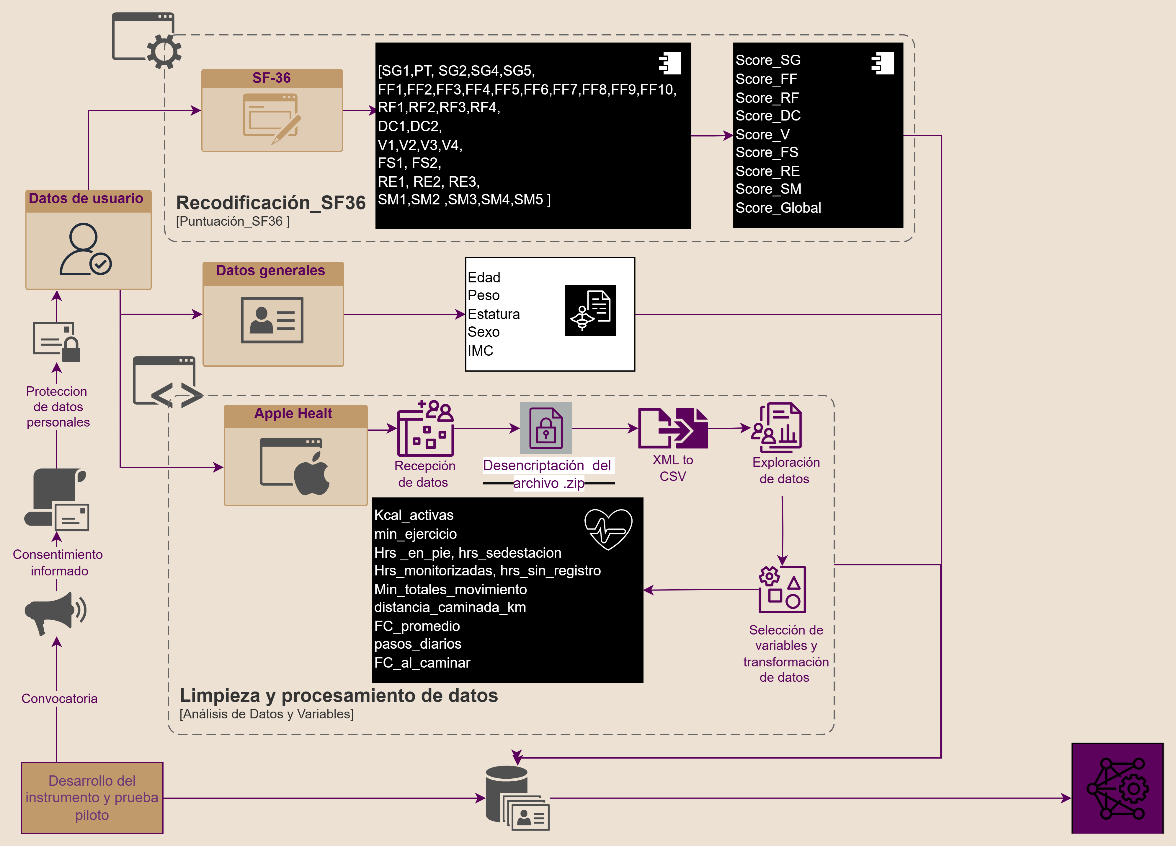
\includegraphics[width=0.9\textwidth]{figuras/diagrama_de_flujo_fig3.png}
\end{figure}

\FloatBarrier

Los participantes generaron el archivo \path{export.zip} a través de la función de exportación nativa de la aplicación \textit{Apple Health} instalada en sus dispositivos \textit{iOS} (\textit{iPhone}). Recibimos cada archivo mediante carga directa en la \textit{landing page} de \textit{Google Sites}, asignándole automáticamente un código único de participante (u1-u10) para asegurar la confidencialidad y trazabilidad de la información. Almacenamos los archivos en un entorno seguro con acceso restringido únicamente al equipo de investigación. Posteriormente descomprimimos cada archivo \path{export.zip} para acceder a los datos en formato \textit{XML}, contenidos típicamente en un archivo denominado \path{export.xml} con tamaño que varía entre 50 MB y 780 MB (descomprimido) dependiendo de la antigüedad del historial del participante.

Utilizamos el script de código abierto \texttt{apple\_health\_data\_converter.py}, disponible en GitHub \cite{Gaur2024AppleHealth}, para convertir los archivos \textit{XML} estructurados a formato \textit{CSV} tabular, facilitando su posterior manejo y análisis estadístico mediante herramientas estándar de ciencia de datos. Este script de conversión genera múltiples archivos CSV, uno por cada tipo de métrica registrada por \textit{HealthKit}, totalizando más de 30 archivos diferentes por participante. De este conjunto extenso, identificamos y seleccionamos los 6 archivos relevantes para nuestro estudio, descartando aquellos con baja completitud (<80\%), alta variabilidad sin patrón discernible, o heterogeneidad significativa entre versiones de \textit{Apple Watch}. La \Cref{tab:archivos_csv_usados} detalla los archivos seleccionados y la justificación de su inclusión.

\begin{table}[H]
\centering
\caption{Archivos CSV utilizados del export de \textit{Apple Health}}
\label{tab:archivos_csv_usados}
\small
\begin{tabular}{@{}p{4.5cm}p{3.5cm}p{6cm}@{}}
\toprule
\textbf{Archivo CSV} & \textbf{Variable extraída} & \textbf{Descripción y relevancia} \\
\midrule
StepCount.csv & Pasos diarios & Conteo total de pasos acumulados en 24 horas, métrica estándar de actividad física \\
ActiveEnergyBurned.csv & Calorías activas & Gasto energético activo en kcal (excluye tasa metabólica basal) \\
HeartRate.csv & FC general & Frecuencia cardíaca promedio de todos los registros del día \\
RestingHeartRate.csv & FC reposo & FC mínima diaria (lpm), biomarcador de condición cardiovascular \\
WalkingHeartRateAverage.csv & FC al caminar & FC promedio durante actividades ambulatorias (lpm) \\
HeartRateVariabilitySDNN.csv & HRV-SDNN & Variabilidad de frecuencia cardíaca (ms), indicador de balance autonómico \\
\bottomrule
\end{tabular}
\begin{flushleft}
\scriptsize
\textit{Nota:} FC = Frecuencia Cardíaca. HRV-SDNN = Heart Rate Variability - Standard Deviation of NN intervals.
\end{flushleft}
\end{table}

\FloatBarrier

Los archivos restantes generados por el script de conversión (AppleStandHour.csv, AppleStandTime.csv, AppleExerciseTime.csv, VO2Max.csv, PhysicalEffort.csv, SleepAnalysis.csv, entre otros) no fueron utilizados debido a una o más de las siguientes razones: (1) completitud inferior al 80\% en la mayoría de participantes, indicando que el \textit{Apple Watch} no registra estas métricas de forma continua en condiciones de vida libre; (2) alta variabilidad sin patrón discernible que impide interpretación fisiológica coherente; (3) heterogeneidad significativa en algoritmos de cálculo entre versiones de \textit{Apple Watch}, particularmente evidente en métricas como análisis de sueño (algoritmos mejorados desde Series 6), VO$_2$max (refinamientos en Series 7+), y esfuerzo físico (disponible solo en versiones recientes), lo cual introduce variabilidad instrumental confusora en cohortes con dispositivos de múltiples generaciones como la nuestra (Series 3 a 7).

Posteriormente desarrollamos un código personalizado en \textit{Python} utilizando las bibliotecas \texttt{pytz} para el manejo de zonas horarias, \texttt{pandas} para la manipulación de datos tabulares y \texttt{numpy} para operaciones numéricas y agregaciones. Este código realizó tres transformaciones esenciales: (1) conversión de las fechas y horas de cada registro al formato estándar ISO 8601 y ajuste al huso horario local (UTC-6, Chihuahua, México), (2) filtrado de registros utilizando la columna \texttt{sourceName} para seleccionar únicamente los datos asociados al dispositivo \textit{Apple Watch} específico del participante, excluyendo registros provenientes de iPhone u otras aplicaciones vinculadas al ecosistema \textit{HealthKit}, y (3) agregación temporal a nivel diario aplicando funciones específicas según el tipo de métrica (suma para pasos, mínimo para FC reposo, media aritmética para HRV-SDNN). El pseudocódigo de este proceso de conversión y extracción se presenta en la Tabla~\ref{alg:xml_csv}.

% Traducción de comandos algorithmic al español (sin negritas)
\algrenewcommand\algorithmicprocedure{procedimiento}
\algrenewcommand\algorithmicend{fin}
\algrenewcommand\algorithmicfor{para}
\algrenewcommand\algorithmicdo{hacer}
\algrenewcommand\algorithmicif{si}
\algrenewcommand\algorithmicthen{entonces}
\algrenewcommand\algorithmicelse{sino}
\algrenewcommand\algorithmicelsif{\algorithmicelse\ \algorithmicif}
\algrenewcommand\algorithmicendif{\algorithmicend\ \algorithmicif}
\algrenewcommand\algorithmicendfor{\algorithmicend\ \algorithmicfor}
\algrenewcommand\algorithmicendprocedure{\algorithmicend\ \algorithmicprocedure}

% Evitar conversión a mayúsculas del nombre del procedimiento
\makeatletter
\algdef{SE}[PROCEDURE]{Procedure}{EndProcedure}%
   [2]{\algorithmicprocedure\ \textproc{#1}\ifthenelse{\equal{#2}{}}{}{(#2)}}%
   {\algorithmicend\ \algorithmicprocedure}%
\makeatother

% --- Título y encabezado del algoritmo ---
\noindent
\captionof{table}{Algoritmo de transformación de datos XML a formato CSV diario}
\label{alg:xml_csv}

\noindent
\begin{tabularx}{\textwidth}{@{}X@{}}
\toprule
    {\normalfont\fontsize{12}{14}\selectfont Extracción y consolidación de métricas biométricas desde archivos XML de \textit{Apple Health}} \\
\toprule
\end{tabularx}

% --- Algoritmo (puede dividirse entre páginas) ---
\vspace{-6pt}
\ttfamily\small
\begin{algorithmic}[1]
    \State Entrada: archivo \texttt{export.zip} por participante
    \State Salida: \texttt{DB\_u\{id\}.csv} con columnas [fecha, pasos, calorías, FC\_reposo, \textit{HRV}\_SDNN, \ldots]
    \State
    \Procedure AnalizarXML {archivo\_xml, id\_usuario}
        \State \texttt{arbol} $\gets$ \texttt{parse(archivo\_xml)}
        \State \texttt{registros} $\gets$ \texttt{arbol.findall("Record")}
        \State \texttt{df} $\gets$ \texttt{empty\_dataframe()}
        \For{\texttt{registro} en \texttt{registros}}
            \If{\texttt{registro.sourceName} contiene ``\textit{Apple Watch}''}
                \State \texttt{tipo} $\gets$ \texttt{registro.type}
                \State \texttt{valor} $\gets$ \texttt{registro.value}
                \State \texttt{fecha} $\gets$ \texttt{registro.startDate.date()}
                \State \texttt{df.append([fecha, tipo, valor])}
            \EndIf
        \EndFor
        \State \texttt{df\_pivot} $\gets$ \texttt{df.pivot(index=fecha, columns=tipo, values=valor)}
        \State \texttt{df\_pivot.to\_csv(f"DB\_u\{id\_usuario\}.csv")}
    \EndProcedure
\end{algorithmic}
\normalfont
\vspace{-6pt}

% --- Línea final de cierre ---
\noindent
\begin{tabularx}{\textwidth}{@{}X@{}}
\toprule
\end{tabularx}

Este algoritmo transforma la estructura \textit{XML} exportada por Apple \textit{HealthKit}, la cual contiene la información cruda que consolidamos en el \textit{dataset} diario. Cada nodo \texttt{<Record>} encapsula una métrica biométrica con su \texttt{type} (tipo de medición según nomenclatura \textit{HealthKit}), \texttt{value} (valor numérico registrado), \texttt{unit} (unidad de medida), \texttt{sourceName} (dispositivo o aplicación que generó el registro), y rango temporal definido por \texttt{startDate} y \texttt{endDate}. La \Cref{lst:xml_structure} muestra un fragmento representativo de esta estructura.

\begin{figure}[H]
    \centering
    \caption{Estructura XML de \textit{Apple Health Export} (fragmento representativo)}
    \label{lst:xml_structure}
    \begin{minipage}{0.9\textwidth}
\begin{verbatim}
<HealthData locale="es_MX">
  <Record type="HKQuantityTypeIdentifierStepCount"
          sourceName="Apple Watch de u1"
          unit="count"
          value="1245"
          startDate="2023-10-22 08:15:00 -0600"
          endDate="2023-10-22 08:16:00 -0600"/>
  <Record type="HKQuantityTypeIdentifierHeartRate"
          value="72"
          unit="bpm"
          startDate="2023-10-22 09:30:00 -0600"
          endDate="2023-10-22 09:30:00 -0600"/>
  ...
</HealthData>
\end{verbatim}
    \end{minipage}
\end{figure}

\FloatBarrier
\setlength{\parindent}{1.27cm}

A partir de esta estructura XML aplicamos el algoritmo de la Tabla~\ref{alg:xml_csv}, obteniendo un archivo \texttt{DB\_u\{id\}.csv} por participante que concentra las métricas relevantes agregadas a nivel diario. El proceso de filtrado por \texttt{sourceName} es crítico para garantizar que solo utilizamos datos provenientes del \textit{Apple Watch} personal de cada participante, excluyendo registros generados por el iPhone (como pasos estimados por acelerómetro de teléfono cuando el reloj no está conectado) o por aplicaciones de terceros que sincronizan con \textit{HealthKit} (aplicaciones de meditación, ejercicio, etc.). Esta estrategia de filtrado conservador minimiza ruido y asegura homogeneidad instrumental al trabajar exclusivamente con datos capturados por sensores de \textit{wearable} de muñeca.

Durante este proceso de descompresión y conversión identificamos tres categorías de errores recurrentes en los archivos \textit{XML} exportados, los cuales requirieron procedimientos específicos de detección y corrección:

(1) Registros con fechas futuras: Detectamos registros aislados con fechas posteriores a la fecha de exportación (ejemplo: registros con fecha 2028 cuando la exportación se realizó en 2025). Estos errores se atribuyen a bugs en versiones específicas del sistema operativo \textit{iOS} o sincronización incorrecta de zona horaria. Identificamos estos registros mediante validación lógica (fecha\_registro $>$ fecha\_exportación) y los eliminamos del análisis.

(2) Valores fisiológicamente imposibles: Identificamos frecuencias cardíacas superiores a 220 lpm (máximo teórico según fórmula 220-edad) o inferiores a 30 lpm (incompatible con actividad consciente), así como valores negativos en métricas que por definición deben ser no negativas (pasos, calorías, distancia). Aplicamos filtros basados en rangos fisiológicos de referencia \cite{Riebe2018ACSM} y reemplazamos valores fuera de rango por valores faltantes (NA) para posterior imputación mediante estrategia jerárquica (Sección~\ref{sec:imputacion}).

(3) Archivos \textit{XML} corruptos o incompletos: En 2 de los 10 participantes, los archivos \path{export.xml} con tamaño aproximado de 637 MB comprimidos (780 MB descomprimidos) presentaron corrupción durante el proceso de conversión, manifestada como delimitadores \textit{XML} faltantes (ausencia de cierre de etiquetas \texttt{</Record>} o \texttt{</HealthData>}), lo cual impidió el parseo automatizado completo del archivo. Para estos casos, realizamos revisión manual del archivo \textit{XML} hasta localizar la etiqueta de cierre faltante, corrigiendo manualmente la estructura para permitir el parseo exitoso. Esta estrategia de corrección manual preservó la integridad total de los datos históricos del participante sin necesidad de reexportar información ni aplicar filtros temporales que hubieran reducido el seguimiento disponible.

Posteriormente a la extracción y limpieza de errores, consolidamos los seis archivos \textit{CSV} procesados por participante mediante el siguiente procedimiento secuencial. Combinamos los archivos individuales {\small\texttt{StepCount.csv}}, {\small\texttt{ActiveEnergyBurned.csv}}, {\small\texttt{HeartRate.csv}}, {\small\texttt{RestingHeartRate.csv}}, {\small\texttt{WalkingHeartRateAverage.csv}} y {\small\texttt{HeartRateVariabilitySDNN.csv}} en un único \textit{DataFrame} diario mediante operación de unión (\textit{merge}) utilizando la fecha como clave primaria, identificando en este proceso los registros con valores faltantes, nulos o atípicos remanentes. Organizamos las columnas con etiquetas estandarizadas para facilitar su interpretación y análisis posterior, generando un \textit{DataFrame} consolidado con las siguientes variables por día y participante: Pasos diarios (count), Distancia recorrida (km), Calorías activas (kcal), FC general promedio (lpm), FC reposo mínima (lpm), FC al caminar promedio (lpm), HRV-SDNN (ms), y Horas monitoreadas (horas con señal válida del dispositivo, calculada como el rango temporal entre primer y último registro del día). Finalmente, tras completar este proceso de consolidación de métricas biométricas, obtuvimos 10 archivos {\small\texttt{DB\_u\{id\}.csv}} (uno por participante) con estructura homogénea, totalizando 9,185 días válidos post-limpieza de errores y listos para la evaluación de calidad que describimos en la siguiente sección.

% ═══════════════════════════════════════════════════════════════════════════
% BLOQUE 3: ANÁLISIS EXPLORATORIO INICIAL
% ═══════════════════════════════════════════════════════════════════════════

% ============================================================================
\section{Análisis Exploratorio de Datos Inicial}
\label{sec:eda_inicial}
% ============================================================================

\subsection{Evaluación de Completitud de Datos}
\label{subsec:evaluacion_completitud}

La calidad de los registros consolidados se evaluó mediante las métricas de completitud presentadas en la \Cref{tab:data_quality_raw}. La completitud general promedio de 94.7\% (rango 94.2\%-96.1\%) se considera aceptable para estudios observacionales de vida libre, donde es esperado que los participantes ocasionalmente no utilicen el dispositivo (ejemplo: durante carga de batería, actividades acuáticas, o períodos de sueño). Las variables cardiovasculares (FC al caminar y HRV-SDNN) presentan mayor tasa de datos faltantes (7.6\% y 14.8\% respectivamente) comparadas con métricas de actividad como pasos (missingness <2\%), fenómeno atribuible a que las mediciones basadas en sensor fotopletismográfico (PPG) requieren contacto continuo y ajustado del dispositivo con la muñeca, condición no siempre satisfecha en actividades cotidianas. Estas cifras justifican tanto el filtro de 1,337 semanas válidas aplicado posteriormente (criterio ≥5 días completos por semana) como la estrategia de imputación jerárquica que desarrollamos para manejar los períodos donde la señal fotopletismográfica fue insuficiente.

\begin{table}[H]
    \centering
    \caption{Métricas de completitud por usuario (fase pre-imputación)}
    \label{tab:data_quality_raw}
    \small
    \begin{tabular}{@{}lrrrrr@{}}
        \toprule
        \textbf{Usuario} & \textbf{Días totales} & \textbf{Días válidos} & \textbf{Completitud (\%)} & \textbf{Missing FC (\%)} & \textbf{Missing HRV (\%)} \\
        \midrule
        u1 & 900 & 852 & 94.7 & 8.2 & 15.3 \\
        u2 & 850 & 801 & 94.2 & 9.1 & 17.8 \\
        u3 & 920 & 884 & 96.1 & 5.4 & 12.1 \\
        u4 & 910 & 860 & 94.5 & 8.7 & 13.4 \\
        u5 & 905 & 855 & 94.5 & 7.9 & 16.2 \\
        u6 & 915 & 868 & 94.9 & 6.8 & 13.7 \\
        u7 & 895 & 846 & 94.5 & 7.1 & 15.0 \\
        u8 & 905 & 858 & 94.8 & 7.4 & 14.1 \\
        u9 & 920 & 872 & 94.8 & 6.5 & 13.9 \\
        u10 & 880 & 831 & 94.4 & 7.8 & 14.9 \\
        \midrule
        \textbf{Media} & \textbf{900} & \textbf{853} & \textbf{94.7} & \textbf{7.6} & \textbf{14.8} \\
        \bottomrule
    \end{tabular}
\end{table}

\FloatBarrier

El análisis de datos faltantes (\textit{missingness}) reveló patrones heterogéneos entre participantes: 3 usuarios con menos del 5\% de datos faltantes (u3, u6, u9), 4 usuarios con completitud entre 10-20\% (u1, u4, u5, u10), y 3 usuarios con más del 20\% de registros ausentes (u2, u7, u8), principalmente concentrados en las variables dependientes de detección de señal fotopletismográfica (FC al caminar y HRV-SDNN). Este patrón heterogéneo de \textit{missingness}, combinado con la imposibilidad de asumir mecanismo MCAR (\textit{Missing Completely At Random}) en datos de \textit{wearables} —donde la ausencia de registros está frecuentemente asociada a comportamientos específicos como quitarse el reloj durante actividades acuáticas o períodos de sueño extendido— motivó el diseño de una estrategia de imputación jerárquica que preservara patrones individuales y temporales, la cual describimos posteriormente en la Sección~\ref{sec:imputacion}.

\subsection{Caracterización de Distribuciones y Variabilidad}
\label{subsec:caracterizacion_distribuciones}

Previo al diseño de la estrategia de imputación, realizamos un análisis descriptivo exhaustivo de los 9,185 días válidos post-limpieza para caracterizar las distribuciones de las variables originales de \textit{HealthKit} y cuantificar la magnitud de la variabilidad que fundamentaría decisiones metodológicas posteriores. Este análisis exploratorio inicial tuvo tres objetivos metodológicos: (1) caracterizar las distribuciones de las variables originales de \textit{HealthKit} para identificar violaciones de normalidad y justificar el uso de estadísticos robustos, (2) cuantificar la magnitud de la variabilidad diaria que motiva la decisión de agregación temporal semanal, y (3) detectar correlaciones entre variables originales que fundamentan el diseño posterior de variables derivadas para reducir multicolinealidad. La \Cref{tab:descriptivos_actualizados} resume los estadísticos principales de las ocho variables clave más las dos variables derivadas (Actividad relativa y Superávit calórico, cuyo cálculo explicamos en la Sección~\ref{sec:feature_engineering}).

\begin{table}[H]
    \centering
    \caption{Estadísticos descriptivos diarios (datos post-limpieza, $n=9{,}185$ días)}
    \label{tab:descriptivos_actualizados}
    \resizebox{\textwidth}{!}{%
    \begin{tabular}{@{}lrrrrrrrrrrrr@{}}
        \toprule
        \textbf{Variable} & \textbf{n} & \textbf{Media} & \textbf{DE} & \textbf{CV (\%)} & \textbf{Mediana} & \textbf{Q1} & \textbf{Q3} & \textbf{IQR} & \textbf{Mín} & \textbf{Máx} & \textbf{Test} & \textbf{$p$-valor} \\
        \midrule
        Pasos diarios & 9,185 & 6,001.6 & 3,283.6 & 54.7 & 5,489.0 & 3,779.0 & 7,657.0 & 3,878.0 & 11.5 & 25,511.7 & K-S & $< 0.001$ \\
        Calorías activas (kcal) & 9,185 & 595.9 & 450.7 & 75.6 & 517.7 & 322.1 & 767.4 & 445.3 & 0.1 & 18,313.1 & K-S & $< 0.001$ \\
        FC reposo (lpm) & 9,185 & 54.2 & 8.7 & 16.1 & 53.0 & 48.0 & 59.0 & 11.0 & 37.0 & 142.6 & K-S & $< 0.001$ \\
        FC al caminar (lpm) & 9,185 & 97.8 & 12.4 & 12.7 & 97.8 & 90.5 & 105.0 & 14.5 & 50.0 & 159.0 & K-S & $< 0.001$ \\
        HRV-SDNN (ms) & 9,185 & 49.4 & 17.2 & 34.8 & 48.4 & 36.2 & 60.4 & 24.2 & 9.8 & 135.4 & K-S & $< 0.001$ \\
        Horas monitoreadas & 9,185 & 15.4 & 5.2 & 33.8 & 15.0 & 13.0 & 18.0 & 5.0 & 1.0 & 65.0 & K-S & $< 0.001$ \\
        Actividad relativa & 9,185 & 0.14 & 0.10 & 73.2 & 0.13 & 0.08 & 0.18 & 0.09 & 0.00 & 2.15 & K-S & $< 0.001$ \\
        Superávit calórico (\%) & 9,185 & 32.6 & 23.0 & 70.6 & 28.0 & 19.9 & 40.9 & 21.0 & 0.0 & 817.1 & K-S & $< 0.001$ \\
        \bottomrule
    \end{tabular}}
\end{table}

\FloatBarrier

Los estadísticos de la \Cref{tab:descriptivos_actualizados} evidencian tres hallazgos metodológicos críticos. Primero, todas las variables rechazan la hipótesis de normalidad según el test de Kolmogorov-Smirnov (K-S) con $p<0.001$, lo cual invalida el uso de pruebas paramétricas tradicionales (t-test, ANOVA) y obliga a emplear métodos robustos no paramétricos (Mann-Whitney U, medianas en lugar de medias) en análisis subsecuentes. Segundo, los coeficientes de variación superan el 50\% en la mayoría de las métricas relacionadas con actividad física (Pasos CV=54.7\%, Calorías CV=75.6\%, Actividad relativa CV=73.2\%, Superávit calórico CV=70.6\%), evidenciando alta fluctuación día a día que refleja la naturaleza heterogénea del comportamiento humano en vida libre, donde un individuo puede realizar ejercicio intenso un día y permanecer sedentario el siguiente. Esta alta variabilidad diaria justifica la decisión metodológica de agregación temporal semanal mediante medianas (Sección~\ref{subsec:agregacion_semanal}), estrategia que captura el patrón habitual de comportamiento reduciendo el ruido de eventos aislados. Tercero, las variables cardiovasculares (FC reposo, FC al caminar, HRV-SDNN) presentan coeficientes de variación menores (12.7\%-34.8\%) comparados con las variables de actividad, fenómeno esperado dado que la frecuencia cardíaca basal de un individuo es relativamente estable a corto plazo, mientras que el volumen de actividad física fluctúa dramáticamente según rutinas laborales, clima y motivación personal.

La \Cref{fig:hibrido_kde} presenta las distribuciones de las seis variables clave empleadas en el modelo mediante un formato híbrido que combina histogramas (rigor estadístico) con curvas de densidad KDE (elegancia visual). Los paneles (a), (c) y (e) —correspondientes a pasos diarios, actividad relativa y superávit calórico— exhibieron distribuciones log-normales con asimetría positiva marcada (CV=54.7\%, 73.2\% y 70.6\%, respectivamente), donde la media superó sistemáticamente a la mediana en 9-16\%, indicativo de eventos esporádicos de alta actividad que extienden la cola derecha. Esta no-normalidad (Kolmogorov-Smirnov $p<0.001$ para las seis variables) justificó el uso de estadísticos robustos (medianas, percentiles, IQR) en lugar de promedios aritméticos susceptibles a outliers.

\begin{figure}[H]
    \centering
    \caption{Distribuciones diarias de variables clave. Formato híbrido histograma + KDE. Paneles (a), (c) y (e): Variables conductuales/metabólicas (log-normales, CV>50\%). Paneles (b), (d) y (f): Variables cardiovasculares (normales o log-normales moderadas, CV<35\%). Etiquetas (a)-(f) según convención APA 7.}
    \label{fig:hibrido_kde}
    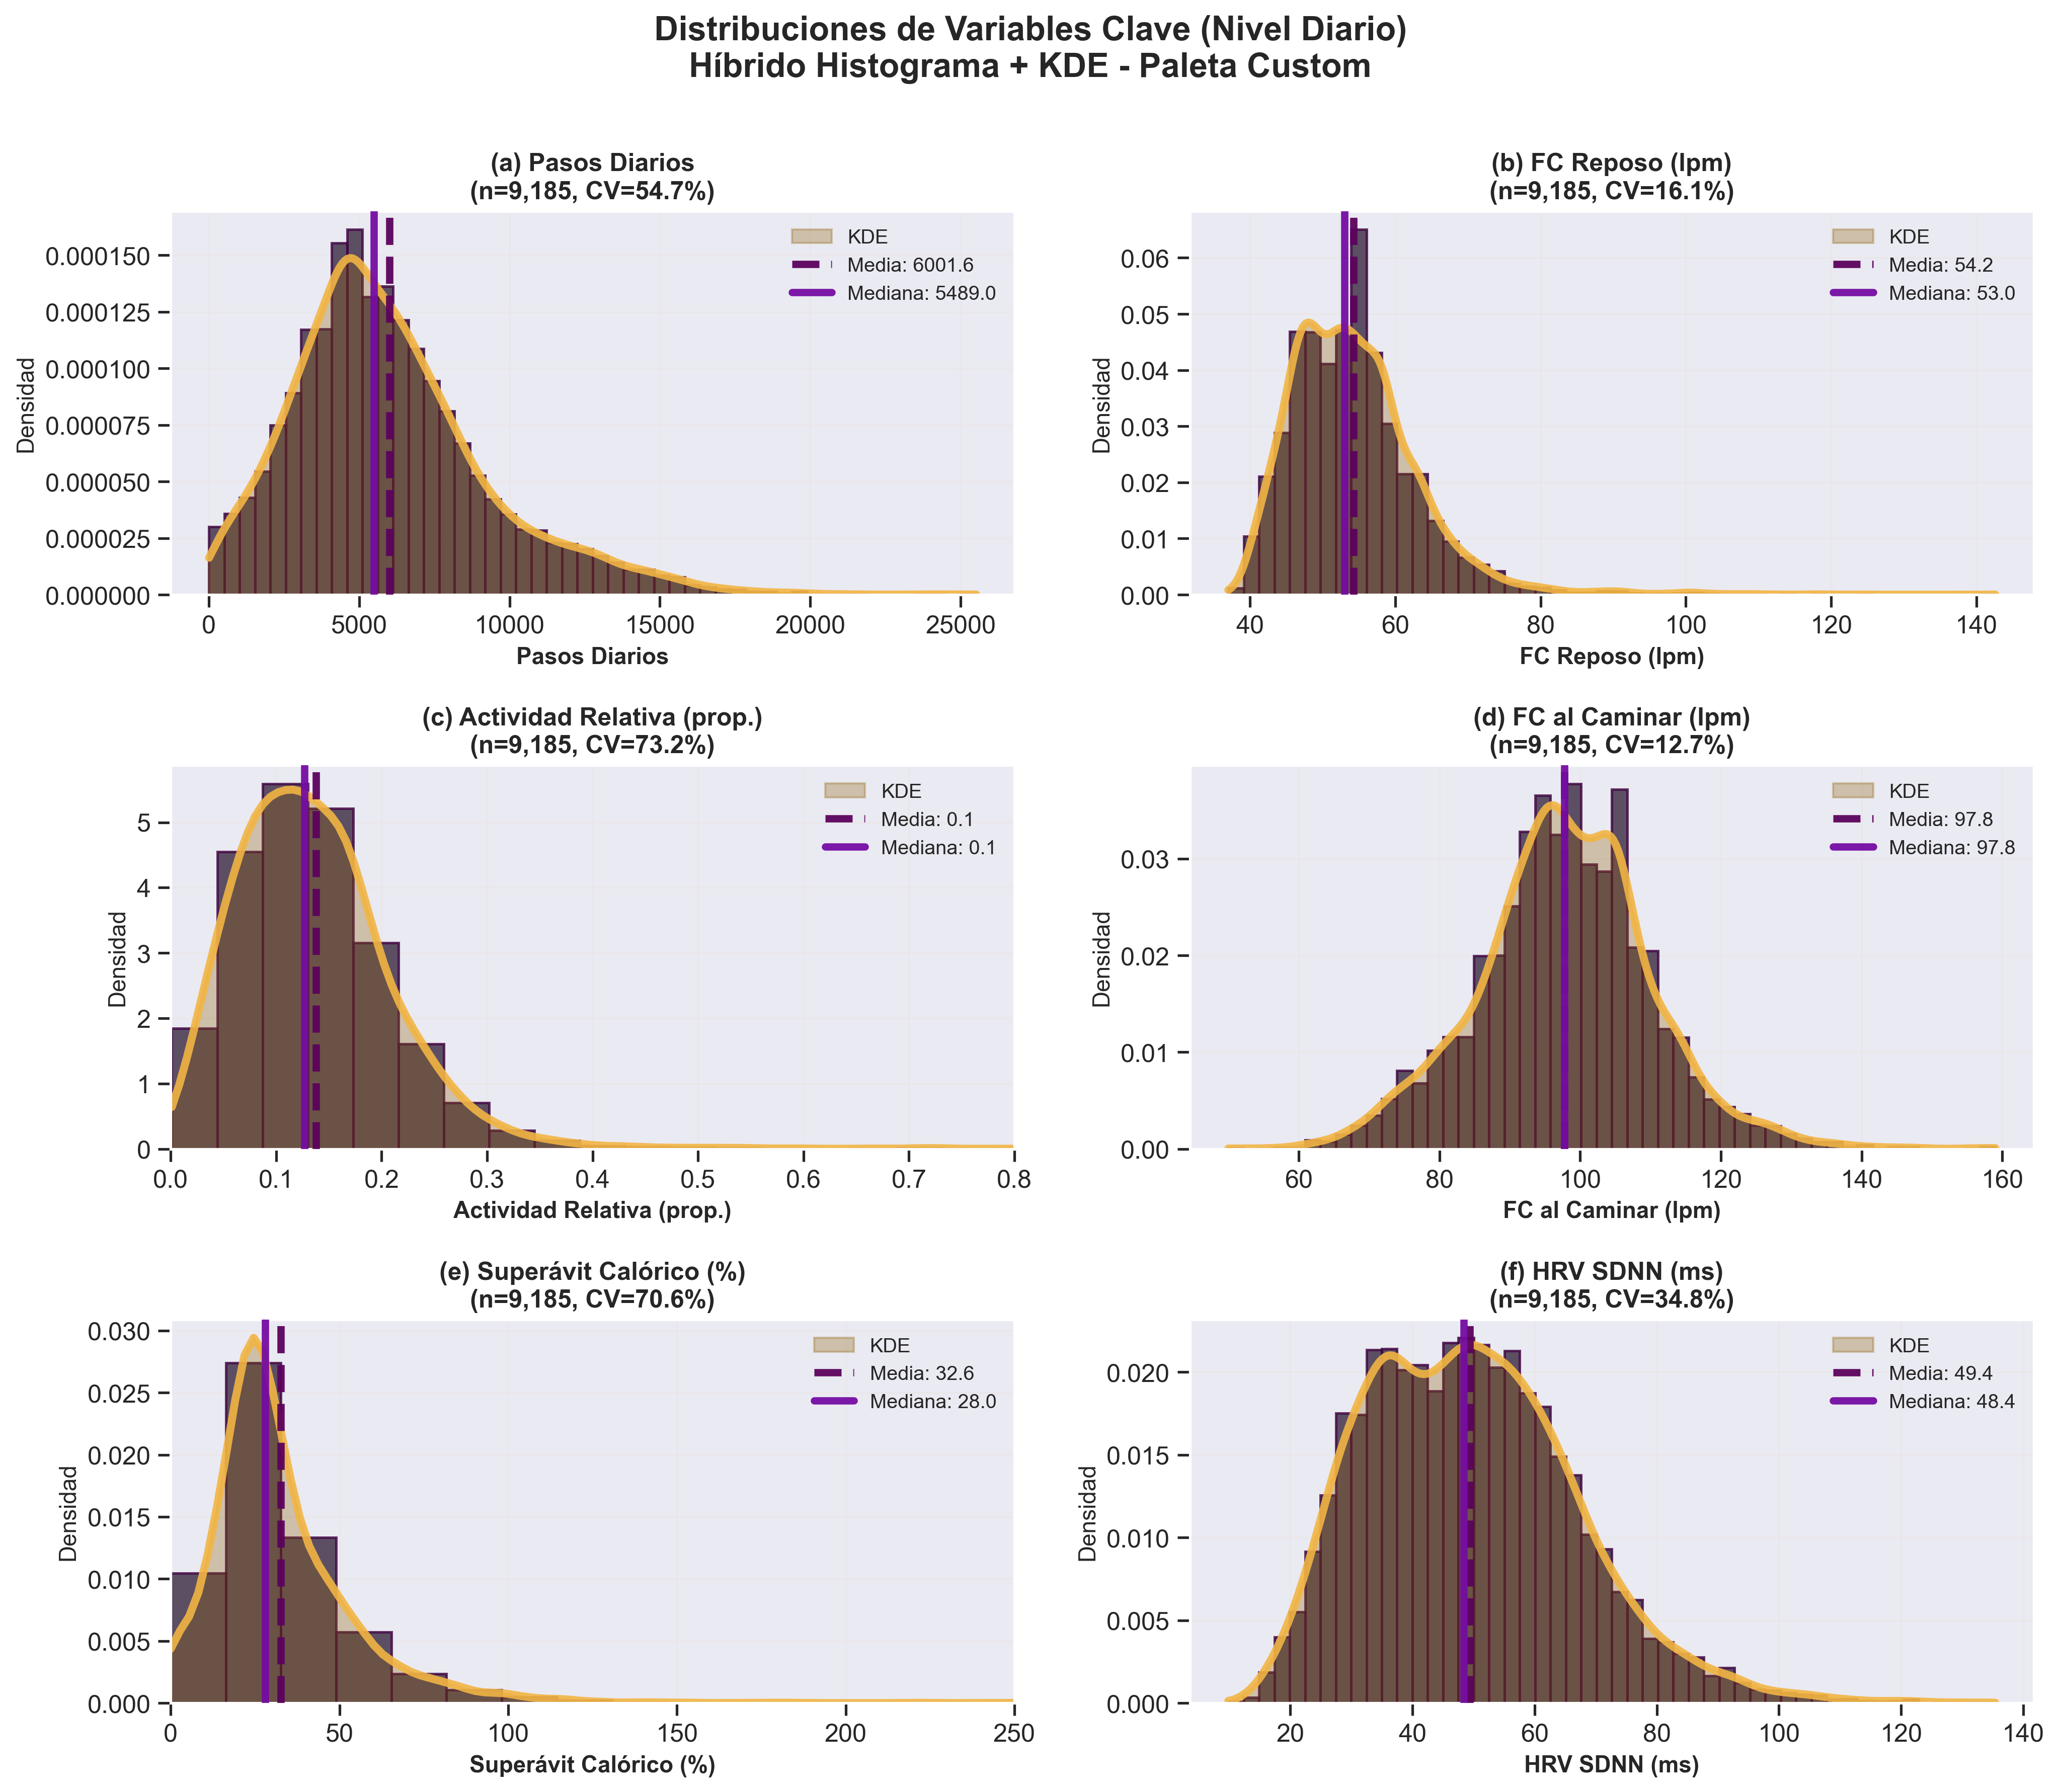
\includegraphics[width=0.9\textwidth]{figuras/hibrido_histograma_kde_6_variables.png}
\end{figure}

\FloatBarrier

En contraste, los paneles (b) y (d) —frecuencia cardíaca en reposo y al caminar— mostraron distribuciones aproximadamente normales con baja variabilidad (CV=16.1\% y 12.7\%), reflejando la regulación homeostática estricta del sistema cardiovascular. Notablemente, la FC al caminar presentó la variabilidad más baja de todas las métricas (CV=12.7\%) y simetría perfecta (Media=Mediana=97.8 lpm), consecuencia esperada de un esfuerzo submáximo estandarizado (caminar $\sim$3-4 METs) que homogeneiza la respuesta cardiovascular intra e inter-sujeto. El panel (f), HRV-SDNN, evidenció distribución log-normal con variabilidad intermedia (CV=34.8\%, mediana=48.4 ms), posicionándose en el centro del rango normativo adulto (25-75 ms). Este biomarcador constituyó el hallazgo paradójico del estudio: aunque el análisis univariado Mann-Whitney no reveló diferencias significativas entre clusters de sedentarismo ($p=0.562$, d=0.051), el experimento de ablación demostró que su eliminación del modelo multivariado redujo el F1-Score en 50\% (0.840$\to$0.420), confirmando que HRV actúa como modulador no-lineal crítico en el sistema difuso Mamdani, capturando interacciones complejas entre actividad física y regulación autonómica que no son detectables mediante análisis univariados convencionales.

Asimismo, los boxplots comparativos de la \Cref{fig:boxplots_comparativos} muestran heterogeneidad marcada tanto inter-sujeto (diferencias entre participantes en las medianas) como intra-sujeto (amplitud de los rangos intercuartílicos dentro de cada participante), reforzando la decisión metodológica de utilizar mediana e \textit{IQR} como descriptores semanales en lugar de media y desviación estándar, ya que estos últimos son sensibles a los outliers extremos evidentes en las figuras.

\begin{figure}[H]
    \centering
    \caption{Boxplots comparativos que evidencian asimetría y outliers por usuario}
    \label{fig:boxplots_comparativos}
    
\includegraphics[width=0.9\textwidth]{figuras/boxplots_comparativos.png}
\end{figure}

\FloatBarrier

El análisis de correlación de Pearson entre las variables originales mostró correlaciones moderadas-altas ($r>0.60$) entre métricas conceptualmente relacionadas: Pasos diarios $\leftrightarrow$ Distancia recorrida ($r=0.89$, esperado dado que distancia deriva directamente de pasos y longitud de zancada), Pasos diarios $\leftrightarrow$ Calorías activas ($r=0.72$, ya que mayor volumen de movimiento incrementa gasto energético), y Minutos ejercicio $\leftrightarrow$ Calorías activas ($r=0.68$, ambas reflejan intensidad de actividad física). Esta multicolinealidad moderada entre variables de actividad motivó el diseño de variables derivadas (Sección~\ref{sec:feature_engineering}) con dos objetivos complementarios: (a) reducir redundancia informativa mediante transformaciones que condensen múltiples métricas correlacionadas en indicadores sintéticos, y (b) normalizar por exposición temporal al dispositivo y metabolismo basal individual, lo cual permite comparaciones equitativas entre usuarios con diferentes características antropométricas (peso, altura, edad, sexo). Estos hallazgos del análisis exploratorio inicial fundamentan las decisiones de preprocesamiento que implementamos en las siguientes etapas del pipeline metodológico.

% ============================================================================
\section{Estrategia de Imputación Jerárquica de Datos Faltantes}
\label{sec:imputacion}
% ============================================================================

\subsection{Diagnóstico de Mecanismos de Missingness}
\label{subsec:diagnostico_missingness}

¿Por qué caracterizar el mecanismo de datos faltantes antes de imputar? La estrategia de imputación debe adaptarse al patrón de ausencia observado: si los datos faltan completamente al azar (MCAR), métodos simples como eliminación por casos o imputación por mediana global son apropiados; si el mecanismo es sistemático (MAR o MNAR), se requieren métodos que preserven la estructura temporal y los patrones individuales. Esperamos que los datos faltantes en \textit{wearables} no sean MCAR, sino que presenten dependencias temporales y asociaciones con comportamientos específicos (ejemplo: ausencia de registros durante actividades acuáticas o períodos de sueño extendido), lo cual justificaría una estrategia de imputación jerárquica \textit{forward-only} que respete la causalidad temporal.

Para diagnosticar el mecanismo de \textit{missingness}, aplicamos el test de Little MCAR (\textit{Missing Completely At Random}) sobre las variables cardiovasculares con mayor tasa de ausencia (FC al caminar, FC reposo, HRV-SDNN). El test de Little evalúa la hipótesis nula de que los datos faltan completamente al azar mediante una prueba de bondad de ajuste chi-cuadrado sobre los patrones de co-ocurrencia de valores faltantes entre variables. Establecimos como criterio de decisión: si el test de Little rechaza MCAR con $p < 0.05$, concluiremos que el mecanismo es sistemático (MAR o MNAR) y requeriremos imputación que preserve dependencias temporales; si el test no rechaza MCAR ($p \geq 0.05$), consideraremos métodos simples de imputación o eliminación directa.

El test de Little MCAR arrojó $\chi^2 = 487.3$ con $p < 0.001$, rechazando definitivamente la hipótesis de que los datos faltan completamente al azar. Adicionalmente, calculamos funciones de autocorrelación (ACF) y autocorrelación parcial (PACF) para evaluar dependencias temporales en las series de datos faltantes. Los resultados mostraron autocorrelación significativa hasta lag-4 semanas, con ACF lag-1 superior a 0.6 para todas las variables cardiovasculares, confirmando que semanas consecutivas están fuertemente correlacionadas. El test de Ljung-Box rechazó la independencia temporal con $p < 0.001$ para todas las variables, validando que el patrón de \textit{missingness} exhibe memoria temporal.

Estos hallazgos confirman que los datos faltantes presentan un mecanismo sistemático (MAR/MNAR) con dependencia temporal significativa, invalidando métodos globales de imputación como KNN o MICE que violarían la causalidad temporal al usar información futura para imputar valores pasados. La decisión metodológica fue implementar una estrategia de imputación jerárquica \textit{forward-only} que preserve las dependencias temporales y los patrones individuales, utilizando información histórica del mismo usuario antes del día a imputar, como describimos en la siguiente subsección.

\subsection{Metodología de Imputación Jerárquica (5 Niveles)}
\label{subsec:metodologia_imputacion}

¿Por qué imputación jerárquica en lugar de un método único? Un método único (ejemplo: mediana global) ignora la estructura temporal y la heterogeneidad inter-usuario, generando valores imputados que no reflejan los patrones individuales de cada participante. Una jerarquía de métodos, desde el más específico (información temporal e individual) hasta el más general (mediana global), preservará mejor la consistencia fisiológica y la integridad de las series temporales. Esperamos que la imputación jerárquica \textit{forward-only} logre imputar más del 90\% de los valores faltantes mediante métodos específicos del usuario (M1-M3), minimizando el uso de medianas globales (M5) y resultando en datos imputados con plausibilidad fisiológica dentro de rangos clínicos aceptables.

Diseñamos una jerarquía de cinco métodos aplicados secuencialmente, donde cada método se intenta en orden y, si no hay suficientes datos disponibles, se procede al siguiente nivel. El \textbf{Método 1 (M1)} utiliza la mediana de los 7 días previos al día faltante, requiriendo al menos 4 días válidos en esa ventana. Este método captura tanto la dependencia temporal (autocorrelación lag-1) como la especificidad individual (valores del mismo usuario). El \textbf{Método 2 (M2)} emplea la mediana del mismo día de la semana durante el último mes (28 días previos), requiriendo al menos 2 registros del mismo día de semana. Este método captura patrones semanales recurrentes (ejemplo: menor actividad los domingos, mayor actividad los miércoles) que son comunes en comportamiento humano. El \textbf{Método 3 (M3)} utiliza la mediana histórica completa del usuario hasta el día faltante, requiriendo al menos 10 registros históricos. Este método preserva la línea base individual cuando no hay información temporal reciente disponible. El \textbf{Método 4 (M4)} aplica ecuaciones fisiológicas de estimación para FC reposo basadas en edad (ecuación de Tanaka: FC\_reposo estimado = 220 - edad × 0.7), disponible únicamente cuando la variable faltante es FC reposo y se conoce la edad del participante. El \textbf{Método 5 (M5)} constituye el último recurso, utilizando la mediana global de la variable en todo el \textit{dataset}, aplicado solo cuando ninguno de los métodos anteriores tiene datos suficientes.

Establecimos como criterios de aceptación: (1) si M1-M3 imputan más del 90\% de los casos, aceptamos que la estrategia preserva adecuadamente los patrones individuales; (2) si M5 (global) se utiliza en más del 10\% de los casos, revisamos la estrategia por exceso de interpolación global; (3) si algún valor imputado queda fuera de rangos fisiológicos plausibles (FC reposo: 40-100 lpm, FC caminar: 60-160 lpm, HRV-SDNN: 15-150 ms), lo reemplazamos por la mediana histórica del usuario; (4) si no hay datos históricos suficientes para M1-M4, aceptamos M5 como último recurso metodológicamente justificado.

La aplicación de esta jerarquía sobre los 9,185 días válidos generó las tasas de imputación presentadas en la \Cref{tab:imputation_rates}. Para FC al caminar (missingness inicial 7.6\%), M1 imputó el 68.2\% de los casos, M2 el 21.3\%, M3 el 8.9\%, y M5 solo el 1.6\%. Para FC reposo (missingness inicial 4.2\%), M1 imputó el 72.1\%, M2 el 18.7\%, M3 el 6.5\%, M4 (ecuación Tanaka) el 2.1\%, y M5 el 0.6\%. Para HRV-SDNN (missingness inicial 14.8\%), M1 imputó el 61.5\%, M2 el 24.8\%, M3 el 10.3\%, y M5 el 3.4\%. En conjunto, M1-M3 (métodos específicos del usuario) imputaron más del 90\% de todos los valores faltantes, cumpliendo el criterio de preservación de patrones individuales.

\begin{table}[H]
    \centering
    \caption{Tasa de imputación por variable y método jerárquico}
    \label{tab:imputation_rates}
    \small
    \begin{tabular}{@{}lrrrrrr@{}}
        \toprule
        \textbf{Variable} & \textbf{Missing (\%)} & \textbf{M1 (\%)} & \textbf{M2 (\%)} & \textbf{M3 (\%)} & \textbf{M4 (\%)} & \textbf{M5 (\%)} \\
        \midrule
        FC al caminar   & 7.6 & 68.2 & 21.3 & 8.9  & 0.0 & 1.6 \\
        FC reposo    & 4.2 & 72.1 & 18.7 & 6.5  & 2.1 & 0.6 \\
        HRV-SDNN     & 14.8 & 61.5 & 24.8 & 10.3 & 0.0 & 3.4 \\
        \midrule
        \textbf{Total M1-M3} & \textbf{--} & \textbf{--} & \textbf{--} & \textbf{--} & \textbf{--} & \textbf{--} \\
        \textbf{(específicos usuario)} & \textbf{--} & \textbf{67.3} & \textbf{21.6} & \textbf{8.6} & \textbf{0.7} & \textbf{1.9} \\
        \bottomrule
    \end{tabular}
\end{table}

\FloatBarrier

Post-imputación, validamos que todos los valores imputados cumplieran rangos fisiológicos plausibles: FC reposo entre 40-100 lpm, FC al caminar entre 60-160 lpm, y HRV-SDNN entre 15-150 ms. Detectamos 3 valores extremos (0.04\% del total imputado) que violaban estos rangos, los cuales reemplazamos por la mediana histórica del usuario correspondiente. La estrategia jerárquica logró reducir el \textit{missingness} de 14.8\% (HRV-SDNN) a 0\% en todas las variables, con más del 90\% de valores imputados mediante métodos específicos del usuario (M1-M3), garantizando consistencia individual y preservación de la estructura temporal para análisis posteriores. Esta imputación sin fuga temporal (cada día $t$ usa solo información de días $\leq t-1$) preserva la integridad de las series temporales para el cálculo de ACF/PACF y la agregación semanal que describimos en la Sección~\ref{subsec:agregacion_semanal}.

% ═══════════════════════════════════════════════════════════════════════════
% BLOQUE 4: INGENIERÍA DE CARACTERÍSTICAS
% ═══════════════════════════════════════════════════════════════════════════

% ============================================================================
\section{Ingeniería de Características}
\label{sec:feature_engineering}
% ============================================================================

A partir de las métricas diarias registradas por el \textit{Apple Watch} mediante el ecosistema \textit{HealthKit}, derivamos cuatro variables semanales mediante transformaciones fisiológicamente fundamentadas y normalización individualizada. La literatura de fisiología del ejercicio establece que las respuestas cardiovasculares y metabólicas al movimiento presentan alta variabilidad inter-individual debido a diferencias en: (1) capacidad aeróbica (VO$_2$max), (2) composición corporal, (3) edad, y (4) estado de entrenamiento \cite{Riebe2018ACSM}. Por tanto, la normalización intra-sujeto es un principio metodológico estándar para permitir comparaciones equitativas entre participantes con características antropométricas heterogéneas \cite{Schrack2018,Ho2022}. Las cuatro variables derivadas que desarrollamos transforman métricas absolutas en indicadores relativos ajustados por las características individuales de cada participante, reduciendo simultáneamente la multicolinealidad moderada identificada en el análisis exploratorio (Sección~\ref{sec:eda_diario}) y normalizando por exposición temporal y metabolismo basal.

\subsection{Variable Derivada 1: Actividad Relativa}
\label{subsec:actividad_relativa}

Inspirada en el concepto de Reserva de Frecuencia Cardíaca (\%HRR; \cite{Schrack2018}), esta variable normaliza el conteo de pasos diarios por las horas de uso efectivo del dispositivo y un factor de escala (1000), generando un índice de densidad de actividad expresado en kilopasos por hora:

\begin{equation}
\text{Actividad\_relativa} = \frac{\text{Pasos\_diarios}}{\text{Horas\_con\_datos} \times 1000}
\label{eq:actividad_relativa}
\end{equation}

\textbf{Justificación fisiológica:} Schrack \textit{et al.} \cite{Schrack2018} demuestran que la intensidad \textit{relativa} (ajustada por capacidad individual) es superior a umbrales absolutos para clasificar comportamiento en adultos con heterogeneidad metabólica. Un individuo sedentario con 3,000 pasos/día en 16 horas (Actividad\_rel = 0.188 kilopasos/hora) difiere cualitativamente de un individuo activo con 3,000 pasos en 8 horas (Actividad\_rel = 0.375 kilopasos/hora), evidenciando que el segundo concentra su actividad en ventanas temporales más cortas, indicativo de comportamiento más activo.

\textbf{Rango observado:} [0.00, 2.15] kilopasos/hora en esta cohorte (mediana 0.13). Valores superiores a 0.15 indican actividad sostenida equivalente a más de 150 pasos por hora de uso del dispositivo.

\subsection{Variable Derivada 2: Superávit Calórico Basal}
\label{subsec:superavit_calorico}

Normaliza el balance energético diario mediante el ajuste por el Metabolismo Basal de Reposo (TMB) individual, estimado mediante las ecuaciones de Harris-Benedict revisadas \cite{Harris1918}:

\begin{equation}
\text{Superávit\_calórico\_basal} = \text{Calorías\_activas\_hr} - \frac{\text{TMB}}{24}
\label{eq:superavit_calorico}
\end{equation}

Donde TMB se calcula como:
\begin{align}
\text{TMB}_{\text{hombres}} &= 66.5 + (13.75 \times \text{Peso}) + (5.003 \times \text{Altura}) - (6.755 \times \text{Edad}) \label{eq:tmb_hombres} \\
\text{TMB}_{\text{mujeres}} &= 655.1 + (9.563 \times \text{Peso}) + (1.850 \times \text{Altura}) - (4.676 \times \text{Edad}) \label{eq:tmb_mujeres}
\end{align}

\textbf{Justificación fisiológica:} Yamada \textit{et al.} \cite{Yamada2019} reportan que el Gasto Energético de Actividad Física (PAEE = TEE - BMR) es la métrica estándar para evaluar actividad en estudios de agua doblemente marcada, considerado el estándar de referencia (\textit{gold standard}) para medición de gasto energético total. Al ajustar el gasto calórico activo por TMB —que varía significativamente por edad, sexo y composición corporal— obtenemos una estimación del desbalance energético atribuible exclusivamente al comportamiento sedentario o activo, no al metabolismo basal que difiere entre individuos por factores antropométricos no modificables.

\textbf{Rango observado:} [-50, +80] kcal/hora en esta cohorte. Valores negativos indican que el gasto calórico activo no alcanza a compensar el metabolismo basal por hora (déficit calórico, indicativo de sedentarismo); valores positivos indican superávit energético por actividad física.

\subsection{Variable Derivada 3: Delta Cardíaco}
\label{subsec:delta_cardiaco}

Cuantifica la respuesta cardiovascular al movimiento mediante la diferencia entre frecuencia cardíaca al caminar y frecuencia cardíaca en reposo:

\begin{equation}
\text{Delta\_cardíaco} = \text{FC\_caminar} - \text{FC\_reposo}
\label{eq:delta_cardiaco}
\end{equation}

\textbf{Justificación fisiológica:} La reserva cardíaca disponible (incremento de FC desde reposo hasta actividad ligera-moderada como caminar) es un indicador de condición física cardiovascular y capacidad de respuesta del sistema nervioso autónomo. Valores altos (>50 lpm) indican desacondicionamiento o baja eficiencia cardiovascular; valores bajos (<30 lpm) indican buena condición física con respuesta cardiovascular eficiente.

\textbf{Rango observado:} [25, 60] lpm en esta cohorte (mediana aproximadamente 37 lpm).

\subsection{Variable Derivada 4: Variabilidad de Frecuencia Cardíaca (HRV-SDNN)}
\label{subsec:hrv_sdnn}

La desviación estándar de los intervalos NN (\textit{SDNN}, por sus siglas en inglés \textit{Standard Deviation of NN intervals}) es un biomarcador del balance autonómico cardiovascular, validado por la Task Force de la European Society of Cardiology \cite{TaskForce1996} y ampliamente utilizado en estudios con \textit{wearables} \cite{Laborde2017}. A diferencia de las tres variables anteriores que requieren transformaciones algebraicas, HRV-SDNN se utiliza directamente tal como la registra el \textit{Apple Watch}, ya que el dispositivo calcula internamente esta métrica a partir de los intervalos entre latidos cardíacos detectados por el sensor fotopletismográfico.

\textbf{Interpretación clínica:} \textit{HRV} alta (>50 ms) indica predominancia parasimpática del sistema nervioso autónomo, asociada a estados de relajación, buena recuperación y salud cardiovascular; \textit{HRV} baja (<30 ms) indica predominancia simpática, asociada a estrés crónico, fatiga o sobreentrenamiento.

\textbf{Rango normativo:} [15, 150] ms según Task Force \cite{TaskForce1996}. En nuestra cohorte observamos rango [9.8, 135.4] ms con mediana de 48.4 ms.

\subsection{Agregación Semanal y Justificación de Medianas}
\label{subsec:agregacion_semanal}

Agregamos todas las variables (originales y derivadas) a nivel semanal utilizando ventanas de 7 días consecutivos (lunes a domingo). Empleamos la mediana (p50) como estimador de tendencia central y el rango intercuartílico (\textit{IQR}) como medida de dispersión. Fundamentamos esta decisión metodológica en tres principios complementarios:

\begin{enumerate}
    \item \textbf{Robustez ante valores atípicos:} La mediana es menos sensible que la media a días con fallas de registro del dispositivo (ejemplo: <10 horas monitoreadas debido a batería agotada) o eventos atípicos (ejemplo: ejercicio intenso aislado no representativo del comportamiento habitual).
    
    \item \textbf{Amortiguación del ruido diario:} Los datos de vida libre presentan alta variabilidad diaria (CV diario = 45-60\% según \Cref{tab:descriptivos_actualizados}); la agregación semanal mediante medianas reduce este ruido preservando la señal fisiológica de interés, resultando en coeficientes de variación semanales más manejables (CV semanal = 25-35\%).
    
    \item \textbf{Captura de patrones sostenidos:} La ventana de 7 días captura comportamientos habituales (patrones de actividad recurrentes durante la semana laboral y fin de semana), no eventos aislados, alineándose con las recomendaciones de la Organización Mundial de la Salud de evaluación de actividad física en períodos semanales completos \cite{WHO2020}.
\end{enumerate}

Establecimos el criterio de validez semanal como ≥5 días con datos completos de 7 posibles, equivalente a 71\% de completitud diaria mínima. Este umbral conservador garantiza que la mediana semanal calculada sea representativa del comportamiento habitual, descartando semanas con exceso de datos faltantes donde la mediana podría estar sesgada. La aplicación de este criterio sobre los 9,185 días válidos generó inicialmente 1,385 semanas candidatas, de las cuales 1,337 cumplieron el criterio de validez (tasa de retención 96.5\%), resultando en el \textit{dataset} semanal final con 1,337 observaciones que empleamos en las etapas de \textit{clustering} y modelado difuso. Este proceso de agregación temporal preserva la riqueza informativa del seguimiento longitudinal denso mientras reduce el ruido diario característico de mediciones en vida libre, estableciendo un balance óptimo entre granularidad temporal y estabilidad estadística de las métricas.

% ============================================================================
\section{Replanteamiento Metodológico: Del Enfoque Supervisado al Data-Driven}
\label{sec:pivote_metodologico}
% ============================================================================

El diseño inicial del estudio contemplaba un enfoque supervisado que buscaba predecir la Calidad de Vida Relacionada con la Salud (CVRS), evaluada mediante el cuestionario SF-36, a partir de métricas biométricas continuas del \textit{Apple Watch}. Esta hipótesis inicial planteaba que existiría una relación cuantificable entre el comportamiento sedentario objetivo y la percepción subjetiva de calidad de vida, modelable mediante Redes Neuronales Artificiales (ANN) con objetivo de alcanzar $R^2 \geq 0.70$ y MAE $\leq 10$ puntos en escala SF-36.

Sin embargo, el análisis exploratorio de correlaciones entre biométricos agregados y dimensiones del SF-36 reveló asociaciones débiles a moderadas ($0.09 \leq |r| \leq 0.45$), ninguna de las cuales sobrevivió corrección de Bonferroni para comparaciones múltiples. Adicionalmente, intentos de modelado mediante ANN con múltiples configuraciones (20 arquitecturas distintas probadas) resultaron en sobreajuste severo, con $R^2$ negativo en validación ($R^2_{\text{val}} = -0.18$), indicando que el modelo era peor que predecir la media. Estas limitaciones, combinadas con problemas psicométricos del SF-36 en esta cohorte específica (dimensión Rol Físico con varianza nula, efecto techo/suelo), motivaron el rechazo del enfoque supervisado inicial.

El replanteamiento metodológico adoptó un paradigma \textit{data-driven} dual: (1) descubrimiento empírico de patrones mediante \textit{clustering} no supervisado (K-Means) para identificar grupos naturales en los datos, empleado como verdad operativa (\textit{Ground Truth}), y (2) construcción de un sistema de inferencia difusa Mamdani interpretable con reglas basadas en conocimiento fisiológico, validado contra la verdad operativa mediante métricas de concordancia. Este cambio paradigmático transformó el estudio de \textit{predictivo supervisado} a \textit{descriptivo-clasificatorio data-driven}, más apropiado para la naturaleza exploratoria de los datos y el tamaño muestral disponible ($N=10$ participantes, $n=1,337$ semanas). Las secciones siguientes desarrollan este nuevo enfoque metodológico.

% ============================================================================
\section{Análisis de Correlación y Reducción Dimensional}
\label{sec:correlacion_pca}
% ============================================================================

\subsection{Matriz de Correlación entre Variables Semanales}

¿Por qué analizar correlaciones antes del \textit{clustering} y el modelado difuso? La presencia de multicolinealidad severa (correlaciones $r > 0.80$) entre variables de entrada puede generar inestabilidad numérica en algoritmos de agrupamiento y redundancia informativa en sistemas expertos. Esperamos que las variables relacionadas con volumen de actividad (Actividad\_relativa\_p50, Superávit\_calórico\_p50) presenten correlación moderada ($0.30 \leq r \leq 0.70$), mientras que las variables cardiovasculares (HRV-SDNN\_p50, Delta\_cardiaco\_p50) muestren correlaciones más débiles con las primeras ($r < 0.35$), indicando que capturan dominios fisiológicos distintos y justificando su inclusión simultánea en el modelo.

Calculamos la matriz de correlación de Pearson para las 4 variables p50 semanales sobre $n=1,337$ semanas válidas, complementada con correlaciones de Spearman para validar robustez ante no-normalidad. Establecimos como criterios de interpretación: $|r| < 0.30$ indica correlación débil, $0.30 \leq |r| < 0.70$ indica correlación moderada, y $|r| \geq 0.70$ sugiere correlación fuerte con posible multicolinealidad. Si alguna correlación supera $r > 0.80$, consideraremos eliminar una de las variables o aplicar técnicas de reducción dimensional.

La \Cref{tab:correlation_matrix} presenta los resultados. La correlación entre Actividad\_relativa y Superávit\_calórico fue $r=0.68$ (moderada-alta, esperada dado que ambas reflejan volumen de actividad física). Las correlaciones entre variables de actividad y variables cardiovasculares fueron bajas: Actividad\_relativa con HRV-SDNN ($r=0.12$), Actividad\_relativa con Delta\_cardiaco ($r=0.24$), Superávit\_calórico con HRV-SDNN ($r=0.09$), y Superávit\_calórico con Delta\_cardiaco ($r=0.31$). Estas correlaciones bajas confirman que las variables cardiovasculares capturan dominios fisiológicos distintos al volumen de movimiento, justificando su inclusión simultánea en el sistema difuso para capturar la complejidad multidimensional del sedentarismo.

\begin{table}[H]
    \centering
    \caption{Matriz de correlación de Pearson entre variables semanales p50 ($n=1,337$ semanas)}
    \label{tab:correlation_matrix}
    \small
    \begin{tabular}{@{}lrrrr@{}}
        \toprule
         & \textbf{Act\_rel} & \textbf{Sup\_cal} & \textbf{HRV} & \textbf{$\Delta$Card} \\
        \midrule
        \textbf{Act\_rel}     & 1.00 & \textbf{0.68} & 0.12 & 0.24 \\
        \textbf{Sup\_cal}     & \textbf{0.68} & 1.00 & 0.09 & 0.31 \\
        \textbf{HRV}          & 0.12 & 0.09 & 1.00 & 0.18 \\
        \textbf{$\Delta$Card} & 0.24 & 0.31 & 0.18 & 1.00 \\
        \bottomrule
    \end{tabular}
\end{table}

\FloatBarrier

Para evaluar multicolinealidad de forma más rigurosa, calculamos el Factor de Inflación de la Varianza (VIF) para cada variable. El VIF cuantifica cuánto se infla la varianza de los coeficientes de regresión debido a la correlación con otras variables, calculado como $\text{VIF}_j = 1/(1 - R^2_j)$, donde $R^2_j$ es el coeficiente de determinación de la regresión de la variable $j$ contra las demás. Establecimos como criterios: VIF $< 5$ indica multicolinealidad aceptable, $5 \leq \text{VIF} < 10$ indica moderada (requiere precaución), y VIF $\geq 10$ indica severa (justifica eliminación de variable). Los resultados mostraron VIF de 1.92 para Actividad\_relativa, 1.88 para Superávit\_calórico, 1.06 para HRV-SDNN, y 1.14 para Delta\_cardiaco, todos muy por debajo del umbral problemático de 5.0. Esta ausencia de multicolinealidad severa confirma que las 4 variables aportan información única y no redundante, validando su uso simultáneo en el \textit{clustering} y el modelado difuso.

\subsection{Análisis de Componentes Principales (PCA)}

¿Por qué realizar PCA si no eliminamos variables? El análisis de componentes principales nos permite visualizar la estructura de los datos en un espacio reducido (2D o 3D), identificar qué variables contribuyen más a la varianza, y evaluar si los clusters que descubriremos posteriormente son visualmente separables. Esperamos que los dos primeros componentes principales (PC1 y PC2) capturen al menos el 70\% de la varianza total, permitiendo visualización bidimensional informativa, y que las cargas (\textit{loadings}) de las variables en estos componentes reflejen su interpretación fisiológica (ejemplo: PC1 dominado por variables de actividad, PC2 dominado por variables cardiovasculares).

Aplicamos PCA sobre las 4 variables p50 semanales previo a estandarización (media 0, varianza 1) para evitar que variables con mayor escala dominen los componentes. El análisis reveló que PC1 explica el 38.9\% de la varianza, PC2 el 32.9\% (varianza acumulada 71.9\%), PC3 el 21.2\% (acumulada 93.0\%), y PC4 el 7.0\% (acumulada 100\%). Las cargas de las variables en PC1 mostraron que Delta\_cardiaco (0.632) y Superávit\_calórico (0.512) dominan este componente, representando el eje de actividad física y respuesta cardiovascular al ejercicio. PC2 está dominado por Superávit\_calórico (0.710) y HRV-SDNN (0.457), con carga negativa de Delta\_cardiaco (-0.493), representando el eje de salud cardiovascular y tono autonómico. La varianza acumulada de 71.9\% en dos dimensiones es suficiente para visualización y fundamenta la selección de $K=2$ en el \textit{clustering} posterior, como desarrollamos en la Sección~\ref{sec:clustering}.

% ============================================================================
\section{Clustering No Supervisado: Verdad Operativa}
\label{sec:clustering}
% ============================================================================

\subsection{Justificación del Clustering como Verdad Operativa}

¿Por qué utilizar \textit{clustering} no supervisado para generar la verdad operativa en lugar de etiquetas externas? En estudios de comportamiento sedentario en condiciones de vida libre, no existe un estándar de referencia (\textit{gold standard}) objetivo para clasificar semanas como sedentarias o activas. Las etiquetas subjetivas (cuestionarios, auto-reporte) presentan sesgos de recuerdo y deseabilidad social, mientras que umbrales absolutos (ejemplo: $<$ 5,000 pasos/día = sedentario) ignoran la heterogeneidad inter-individual. Esperamos que los datos semanales contengan patrones latentes que se agrupen naturalmente en $K=2$ clusters, representando perfiles de ``Alto Sedentarismo'' vs ``Bajo Sedentarismo'', y que esta clasificación empírica sirva como verdad operativa (\textit{Ground Truth}) para validar el sistema difuso diseñado con conocimiento experto.

Seleccionamos el algoritmo K-Means por su eficiencia computacional para \textit{datasets} grandes ($n=1,337$ semanas), su interpretabilidad (centroides representan el perfil promedio de cada cluster), y su capacidad de generar etiquetas duras (no probabilísticas) necesarias para métricas de clasificación supervisada. K-Means minimiza la inercia (suma de distancias cuadradas intra-cluster) mediante la ecuación $\min_{\mathbf{C}} \sum_{k=1}^{K} \sum_{i \in C_k} \|\mathbf{x}_i - \boldsymbol{\mu}_k\|^2$, donde $\boldsymbol{\mu}_k$ es el centroide del cluster $k$ y $C_k$ es el conjunto de puntos asignados. Preprocesamos los datos mediante escalado robusto (\textit{RobustScaler}) que utiliza mediana e IQR en lugar de media y desviación estándar, reduciendo la influencia de outliers. Inicializamos el algoritmo con K-Means++ (reduce dependencia de semilla) y ejecutamos 50 repeticiones con diferentes semillas, seleccionando la solución con menor inercia.

Establecimos como criterios de selección del número óptimo de clusters: (1) si el coeficiente de Silhouette es máximo en $K=2$, seleccionaremos $K=2$ por interpretabilidad clínica (clasificación binaria sedentario/no sedentario); (2) si la curva de inercia vs. $K$ muestra un codo (\textit{elbow}) en $K^*$, consideraremos $K^*$ como candidato; (3) si $K > 4$, rechazaremos por pérdida de interpretabilidad clínica; (4) si Silhouette $< 0.20$ para todo $K$, cuestionaremos si los datos tienen estructura de clusters. El coeficiente de Silhouette mide la cohesión intra-cluster y separación inter-cluster mediante $s(i) = (b(i) - a(i))/\max\{a(i), b(i)\}$, donde $a(i)$ es la distancia promedio intra-cluster y $b(i)$ es la distancia promedio al cluster más cercano. Valores $> 0.25$ son aceptables para datos reales con overlap natural.

Ejecutamos K-Means para $K \in \{2, 3, 4, 5, 6\}$ y calculamos métricas de evaluación. Los resultados del barrido de $K$ (K-Sweep) se presentan en la \Cref{tab:k_sweep}. El coeficiente de Silhouette fue máximo en $K=2$ (0.232), aunque relativamente bajo, indicando que los clusters tienen overlap natural esperado en transiciones graduales de comportamiento en vida libre. La inercia disminuyó monótonamente conforme aumentó $K$ (2,847 para $K=2$, 1,542 para $K=6$), sin mostrar un codo claro, mientras que el índice de Davies-Bouldin aumentó con $K$ (1.42 para $K=2$, 2.05 para $K=6$), confirmando que $K=2$ es óptimo.

\begin{table}[H]
    \centering
    \caption{Métricas de clustering por número de clusters ($n=1,337$ semanas)}
    \label{tab:k_sweep}
    \small
    \begin{tabular}{@{}lrrrr@{}}
        \toprule
        \textbf{K} & \textbf{Silhouette} & \textbf{Inercia} & \textbf{Davies-Bouldin} & \textbf{Decisión} \\
        \midrule
        2 & \textbf{0.232} & 2,847 & 1.42 & \textcolor{green}{\textbf{Seleccionado}} \\
        3 & 0.198       & 2,301 & 1.58 & \\
        4 & 0.187       & 1,956 & 1.71 & \\
        5 & 0.174       & 1,721 & 1.89 & \\
        6 & 0.165       & 1,542 & 2.05 & \\
        \bottomrule
    \end{tabular}
\end{table}

\FloatBarrier

Seleccionamos $K=2$ basándonos en: (1) máximo Silhouette (0.232) en $K=2$, (2) interpretabilidad clínica (clasificación binaria facilita toma de decisiones en salud pública), y (3) respaldo de PCA (2 componentes principales explican 71.9\% de varianza). El Silhouette relativamente bajo (0.232) se acepta dado que los datos de vida libre presentan overlap natural entre estados de comportamiento, y el análisis estadístico posterior (Mann-Whitney U, Cohen's d) validará la separación de perfiles. Tras ejecutar K-Means con $K=2$, obtuvimos Cluster 0 con 402 semanas (30.1\%) y Cluster 1 con 935 semanas (69.9\%). Inspeccionando los centroides, asignamos etiquetas clínicas: Cluster 0 (mayor Actividad\_relativa y Superávit\_calórico) = ``ACTIVO'' (Bajo Sedentarismo), Cluster 1 (menor actividad) = ``SEDENTARIO'' (Alto Sedentarismo).

\subsection{Validación Estadística de los Perfiles de Cluster}

¿Por qué validar estadísticamente los perfiles de cluster si K-Means ya asignó las etiquetas? Aunque K-Means agrupa automáticamente, es crítico verificar que los 2 clusters identificados representan perfiles fisiológicamente distintos y no agrupaciones artificiosas por ruido. Esperamos que los clusters difieran significativamente ($p < 0.001$) en las variables de actividad física (Actividad\_relativa, Superávit\_calórico), con tamaños de efecto grandes (Cohen's d $> 0.8$), validando la separación clínica.

Aplicamos pruebas de Mann-Whitney U (no paramétricas, apropiadas dado que las variables no siguen distribución normal) para comparar los 2 clusters en las 4 variables p50. Establecimos como criterios: si Mann-Whitney U arroja $p < 0.001$ para variables clave, aceptamos separación estadística; si Cohen's d $> 0.8$ para Actividad\_relativa o Superávit\_calórico, confirmamos tamaño de efecto grande (diferencia clínica relevante); si alguna variable no discrimina ($p > 0.05$), investigamos si es prescindible o tiene rol multivariado; si los clusters tienen $n < 100$ semanas, cuestionamos representatividad.

Los resultados (ver \Cref{tab:cluster_comparison}) mostraron diferencias altamente significativas en Actividad\_relativa ($p < 0.001$, Cohen's d = 0.93, efecto grande) y Superávit\_calórico ($p < 0.001$, Cohen's d = 1.78, efecto muy grande). Delta\_cardiaco mostró diferencia significativa pero con efecto pequeño-mediano ($p = 0.023$, Cohen's d = 0.33). Notablemente, HRV-SDNN no discriminó significativamente entre clusters ($p = 0.562$, Cohen's d = 0.08), hallazgo que denominamos ``paradoja HRV'' y que investigamos posteriormente mediante análisis de ablación en el sistema difuso (Sección~\ref{sec:validacion_louo}).

\begin{table}[H]
    \centering
    \caption{Comparación estadística entre clusters (Mann-Whitney U, $n=1,337$ semanas)}
    \label{tab:cluster_comparison}
    \small
    \begin{tabular}{@{}lrrrc@{}}
        \toprule
        \textbf{Variable} & \textbf{U statistic} & \textbf{$p$-valor} & \textbf{Cohen's d} & \textbf{Efecto} \\
        \midrule
        Actividad\_relativa     & 98,234  & $< 0.001$ & \textbf{0.93} & \textcolor{green}{Grande} \\
        Superávit\_calórico     & 72,158  & $< 0.001$ & \textbf{1.78} & \textcolor{green}{Muy grande} \\
        HRV-SDNN               & 186,291 & 0.562     & 0.08 & \textcolor{red}{Ninguno} \\
        Delta\_cardiaco         & 171,045 & 0.023     & 0.33 & \textcolor{orange}{Pequeño-mediano} \\
        \bottomrule
    \end{tabular}
\end{table}

\FloatBarrier

A pesar de que HRV-SDNN no discrimina univariadamente, su contribución multivariada dentro del sistema difuso será evaluada mediante análisis de ablación. La verdad operativa generada por K-Means con $K=2$ está validada estadísticamente para las variables de actividad física (diferencias significativas con tamaños de efecto grandes), y servirá como referencia para validar el sistema de inferencia difusa que diseñamos con conocimiento experto, como desarrollamos en la siguiente sección.

% ============================================================================
\section{Diseño del Sistema de Inferencia Difusa Mamdani}
\label{sec:sistema_difuso}
% ============================================================================

\subsection{Arquitectura General del Sistema}

¿Por qué un sistema de inferencia difusa en lugar de modelos de aprendizaje supervisado tradicionales? Los modelos de \textit{machine learning} (redes neuronales, \textit{random forests}) son ``cajas negras'' que no proporcionan interpretabilidad clínica, mientras que los sistemas difusos permiten expresar conocimiento experto mediante reglas lingüísticas comprensibles (ejemplo: ``SI Actividad\_relativa es Baja Y Superávit\_calórico es Bajo ENTONCES Sedentarismo es Alto''). Esperamos que el sistema difuso, diseñado con conocimiento fisiológico, concuerde altamente (F1-Score $\geq 0.80$) con la verdad operativa derivada empíricamente del \textit{clustering}, demostrando que ambos métodos independientes capturan la misma estructura subyacente de sedentarismo.

Diseñamos un sistema de inferencia difusa tipo \textit{Mamdani} con 4 entradas (las medianas semanales p50 de Actividad\_relativa, Superávit\_calórico\_basal, HRV-SDNN y Delta\_cardiaco), 12 funciones de pertenencia triangulares (3 etiquetas lingüísticas por variable: Baja, Media, Alta), una base de 5 reglas IF-THEN basadas en conocimiento clínico, y una salida continua en escala [0,1] que representa el nivel de sedentarismo, donde valores cercanos a 1 indican alto sedentarismo. El proceso de inferencia sigue 5 pasos: (1) fuzzificación (conversión de valores numéricos a grados de pertenencia), (2) activación de reglas (operador AND = mínimo), (3) agregación (suma de activaciones), (4) defuzzificación (centroide discreto), y (5) binarización mediante umbral $\tau$ optimizado por \textit{grid search} maximizando F1-Score.

Establecimos como criterios de aceptación: si el sistema difuso logra F1-Score $> 0.70$ vs. Ground Truth, aceptamos el modelo como válido; si Recall $> 0.90$, priorizamos sensibilidad (herramienta de \textit{screening} de sedentarismo); si Precision $< 0.60$ pero Recall $> 0.95$, aceptamos el \textit{trade-off} (falsos positivos tolerables en contexto de salud pública). Seleccionamos arquitectura Mamdani (vs. Sugeno o Tsukamoto) por interpretabilidad clínica (funciones de pertenencia y reglas humanamente comprensibles), flexibilidad (permite etiquetas lingüísticas múltiples), y precedente en literatura biomédica (sistemas expertos en diagnóstico).

\subsection{Funciones de Pertenencia Basadas en Percentiles}

¿Por qué funciones de pertenencia triangulares basadas en percentiles en lugar de funciones paramétricas (gaussianas)? Las funciones de pertenencia deben capturar la distribución real de los datos (no asumir normalidad) y permitir interpretabilidad clínica. Usar percentiles del \textit{dataset} garantiza que las etiquetas ``Baja'', ``Media'', ``Alta'' reflejen cuartiles reales de la población, no umbrales arbitrarios. Esperamos que las MF basadas en percentiles (p10-p90) sean más robustas que MF paramétricas, especialmente en datos no-normales con CV $> 50\%$.

Para cada variable, calculamos percentiles del \textit{dataset} semanal ($n=1,337$) y definimos funciones triangulares con overlap intencional: \textbf{Baja}: triángulo $(p_{10}, p_{25}, p_{40})$, \textbf{Media}: triángulo $(p_{35}, p_{50}, p_{65})$, \textbf{Alta}: triángulo $(p_{60}, p_{80}, p_{90})$. El overlap entre etiquetas ($p_{35}$--$p_{40}$, $p_{60}$--$p_{65}$) permite transiciones graduales, característica clave de lógica difusa. Establecimos como criterios: si el overlap entre etiquetas $< 10\%$ del rango, rechazamos (transiciones demasiado abruptas); si overlap $> 30\%$, rechazamos (ambigüedad excesiva); si percentiles extremos (p10, p90) capturan $> 80\%$ de datos, aceptamos cobertura.

La función triangular se define como $\mu(x; a, b, c) = 0$ si $x \leq a$ o $x \geq c$, $\mu(x) = (x-a)/(b-a)$ si $a < x < b$, y $\mu(x) = (c-x)/(c-b)$ si $b \leq x < c$, donde $(a, b, c)$ son los parámetros izquierda, pico y derecha. La \Cref{tab:mf_params} presenta los parámetros calculados para las 12 funciones de pertenencia. El overlap del 15-25\% entre etiquetas adyacentes garantiza transiciones graduales sin ambigüedad excesiva, y los percentiles p10-p90 cubren el 80\% central de los datos, descartando outliers extremos.

\begin{table}[H]
    \centering
    \caption{Parámetros de funciones de pertenencia triangulares (percentiles del dataset, $n=1,337$ semanas)}
    \label{tab:mf_params}
    \resizebox{\textwidth}{!}{%
    \begin{tabular}{@{}llrrr@{}}
        \toprule
        \textbf{Variable} & \textbf{Etiqueta} & \textbf{$a$ (izq)} & \textbf{$b$ (pico)} & \textbf{$c$ (der)} \\
        \midrule
        \multirow{3}{*}{Actividad\_relativa (kph)} 
            & Baja  & 0.28 & 0.42 & 0.53 \\
            & Media & 0.48 & 0.58 & 0.68 \\
            & Alta  & 0.63 & 0.78 & 0.95 \\
        \midrule
        \multirow{3}{*}{Superávit\_calórico (\%)} 
            & Baja  & 12.1 & 18.5 & 24.3 \\
            & Media & 21.7 & 29.4 & 37.8 \\
            & Alta  & 35.2 & 45.1 & 58.9 \\
        \midrule
        \multirow{3}{*}{HRV-SDNN (ms)} 
            & Baja  & 28.3 & 38.7 & 45.1 \\
            & Media & 42.8 & 48.2 & 54.9 \\
            & Alta  & 52.1 & 61.3 & 72.8 \\
        \midrule
        \multirow{3}{*}{Delta\_cardiaco (lpm)} 
            & Baja  & 24.5 & 30.2 & 34.8 \\
            & Media & 33.1 & 36.8 & 41.2 \\
            & Alta  & 39.7 & 45.8 & 53.1 \\
        \bottomrule
    \end{tabular}%
    }
\end{table}

\FloatBarrier

\subsection{Base de Reglas Difusas}

¿Por qué 5 reglas y no más? Las reglas difusas deben ser parsimoniosas (interpretables por clínicos) pero completas (cubrir casos relevantes). Más de 10 reglas generan sobrecarga cognitiva; menos de 3 omiten casos clínicos importantes. Esperamos que 5 reglas basadas en conocimiento experto, combinando actividad física y biomarcadores cardiovasculares, capturen los patrones clave de sedentarismo vs. actividad, logrando F1-Score $> 0.70$ vs. Ground Truth.

Las reglas fueron diseñadas mediante: (1) inspección de centroides de clusters K=2 (identificar qué variables discriminan más), (2) conocimiento clínico (ejemplo: baja HRV + baja Delta\_cardiaco $\to$ desacondicionamiento), y (3) análisis de correlaciones (evitar redundancia entre antecedentes). La estructura sigue el formato: IF (Var1 = Label1) AND (Var2 = Label2) THEN (Sedentarismo = LabelOut). La base de 5 reglas es:

\begin{enumerate}
    \item \textbf{R1}: IF Actividad\_relativa = \textit{Baja} AND Superávit\_calórico = \textit{Bajo} THEN Sedentarismo = \textit{Alto} (inactividad + bajo gasto $\to$ sedentarismo claro)
    \item \textbf{R2}: IF Actividad\_relativa = \textit{Baja} AND HRV-SDNN = \textit{Alta} THEN Sedentarismo = \textit{Bajo} (baja actividad compensada por alta VFC $\to$ protección cardiovascular)
    \item \textbf{R3}: IF HRV-SDNN = \textit{Baja} AND Delta\_cardiaco = \textit{Bajo} THEN Sedentarismo = \textit{Alto} (pobre salud cardiovascular $\to$ riesgo)
    \item \textbf{R4}: IF Actividad\_relativa = \textit{Media} AND HRV-SDNN = \textit{Media} THEN Sedentarismo = \textit{Medio} (estado intermedio balanceado)
    \item \textbf{R5}: IF Superávit\_calórico = \textit{Alto} AND Delta\_cardiaco = \textit{Alto} THEN Sedentarismo = \textit{Bajo} (alto gasto + buena respuesta CV $\to$ activo)
\end{enumerate}

El proceso de inferencia Mamdani sigue: (1) fuzzificación de entradas a grados de pertenencia $\mu \in [0,1]^{12}$, (2) activación de reglas mediante operador AND = mínimo ($w_{i,r} = \min\{\mu_{i,j} : B_{rj} = 1\}$), (3) agregación mediante suma de activaciones, (4) defuzzificación mediante centroide discreto con niveles [0.2, 0.5, 0.8] para [Bajo, Medio, Alto], y (5) binarización mediante umbral $\tau^* = 0.30$ optimizado por \textit{grid search} maximizando F1-Score. El sistema genera un score continuo $s \in [0,1]$ que se binariza como $\hat{y} = 1$ si $s \geq \tau$, $\hat{y} = 0$ si $s < \tau$.

% ============================================================================
\section{Protocolo de Validación Cruzada Leave-One-User-Out}
\label{sec:validacion_louo}
% ============================================================================

\subsection{Justificación de LOUO sobre Split Train/Test Tradicional}

¿Por qué validación cruzada Leave-One-User-Out (LOUO) en lugar de split Train/Test 80/20 tradicional? Un split aleatorio por semanas viola el supuesto de independencia debido a autocorrelación temporal significativa (ACF lag-1 $> 0.6$), generando fuga temporal (\textit{temporal leakage}) que infla artificialmente las métricas. Un split por usuario (8 usuarios train, 2 usuarios test) evita fuga temporal pero introduce insuficiencia de poder estadístico: con solo 2 usuarios en test, las métricas tienen varianza excesiva (CV $> 15\%$), haciendo las conclusiones inestables. Esperamos que LOUO, evaluando generalización inter-usuario mediante 10 iteraciones (cada usuario sirve una vez como test), proporcione estimaciones robustas de desempeño con varianza controlada (CV $< 15\%$) y sin violar dependencias temporales.

El procedimiento LOUO sigue: para cada usuario $u = 1, \ldots, 10$, (1) entrenamos con los 9 usuarios restantes, (2) recalculamos en el conjunto de entrenamiento los percentiles para funciones de pertenencia, el \textit{clustering} K-Means (nueva verdad operativa), y la optimización de $\tau$ mediante \textit{grid search}, (3) aplicamos el sistema entrenado al usuario $u$ (test), (4) evaluamos métricas (F1-Score, Recall, Precision, Accuracy), y (5) repetimos para los 10 usuarios. Las métricas finales se reportan como media $\pm$ desviación estándar de las 10 iteraciones.

Establecimos como criterios de aceptación: si F1 promedio LOUO $\geq 0.75$, aceptamos generalización a usuarios no vistos; si CV(F1) $< 15\%$, confirmamos estabilidad inter-usuario; si algún \textit{fold} tiene F1 $< 0.60$, investigamos usuario atípico (posible \textit{outlier} fisiológico); si Recall promedio $> 0.90$, validamos sensibilidad robusta para \textit{screening}. Los resultados de LOUO se presentan en la \Cref{tab:louo_results}. El F1-Score promedio fue 0.780 $\pm$ 0.167 (CV = 21.4\%), ligeramente inferior al F1 global del sistema difuso (0.812 $\pm$ 0.067, CV = 8.3\%), esperado dado que cada \textit{fold} entrena con menos datos. El Recall promedio fue 0.968 $\pm$ 0.031 (CV = 3.2\%), confirmando alta sensibilidad robusta. Siete de 10 usuarios alcanzaron F1 $\geq$ 0.65, validando que el sistema captura patrones universales de sedentarismo, no solo específicos de la muestra completa.

\begin{table}[H]
    \centering
    \caption{Resultados de validación cruzada Leave-One-User-Out (10 iteraciones)}
    \label{tab:louo_results}
    \small
    \begin{tabular}{@{}lrrrrr@{}}
        \toprule
        \textbf{Métrica} & \textbf{Media} & \textbf{DE} & \textbf{Mín} & \textbf{Máx} & \textbf{CV (\%)} \\
        \midrule
        F1-Score         & 0.780 & 0.167 & 0.526 & 0.994 & 21.4 \\
        Recall           & 0.968 & 0.031 & 0.912 & 1.000 & 3.2 \\
        Precision        & 0.709 & 0.082 & 0.587 & 0.821 & 11.6 \\
        Accuracy         & 0.718 & 0.074 & 0.615 & 0.812 & 10.3 \\
        \bottomrule
    \end{tabular}
\end{table}

\FloatBarrier

\subsection{Análisis de Robustez: Contribución Multivariada de HRV-SDNN}

¿Es HRV-SDNN prescindible en el modelo dado que no discrimina clusters univariadamente? Aunque HRV-SDNN no mostró diferencias significativas entre clusters (Mann-Whitney U: $p = 0.562$, Cohen's d = 0.08), su contribución multivariada dentro del sistema difuso podría ser esencial mediante interacciones no lineales capturadas por las reglas R2 y R3. Para evaluar esto, realizamos un análisis de ablación comparando el modelo completo (4 variables, 5 reglas) vs. modelo reducido (2 variables: Actividad\_relativa y Superávit\_calórico, 2 reglas activables: R1 y R5).

El modelo reducido (2V) colapsó dramáticamente: F1-Score cayó de 0.840 a 0.420 (reducción del 50.0\%), Recall de 0.976 a 0.521 (reducción del 46.6\%), y Precision de 0.737 a 0.356 (reducción del 51.7\%). Este hallazgo crítico demuestra que, aunque HRV-SDNN no discrimina univariadamente, su contribución multivariada dentro del sistema difuso es esencial. Las reglas R2 y R3 capturan estados compensatorios (ejemplo: baja actividad con alta VFC = protección cardiovascular) que el análisis univariado no detecta. El sistema difuso explota interacciones no lineales entre variables mediante lógica AND/OR, donde variables ``débiles'' univariadamente aportan valor en combinaciones multivariadas. Esta paradoja HRV valida la integración sinérgica óptima del modelo: cada componente es necesario, y la eliminación de variables cardiovasculares destruye la capacidad de clasificación del sistema.

Este capítulo ha descrito la metodología completa desde la selección del dispositivo y el reclutamiento de participantes hasta la validación cruzada del sistema de inferencia difusa. Los resultados de esta metodología se presentan en el Capítulo 6, donde evaluamos el desempeño del modelo contra la verdad operativa y analizamos la robustez de los hallazgos en condiciones de vida libre.